\chapter{Iteration 3 (FYP-2 Mid)}
\label{ch:iter3}

The first iteration is expected to be completed by the midterm of the FYP-2.
This chapter will have some of the artifacts based on system design. The requirements analysis section is same for all the systems while the design may vary. There may have two types of designs the structural design or . First section is for the structural design.


\section{FYP-2 Mid}
\textbf{Objectives for FYP-2 Mid}
	\begin{itemize}
		\item Basic tools
		\item Medicines 
		\item User movements
		\item Grabbing Tools
	\end{itemize}
\newpage
\subsection{Tools and Medicines}
\text{Some basic tools and medicines for practice.}
\begin{figure}[h]
	\centering
	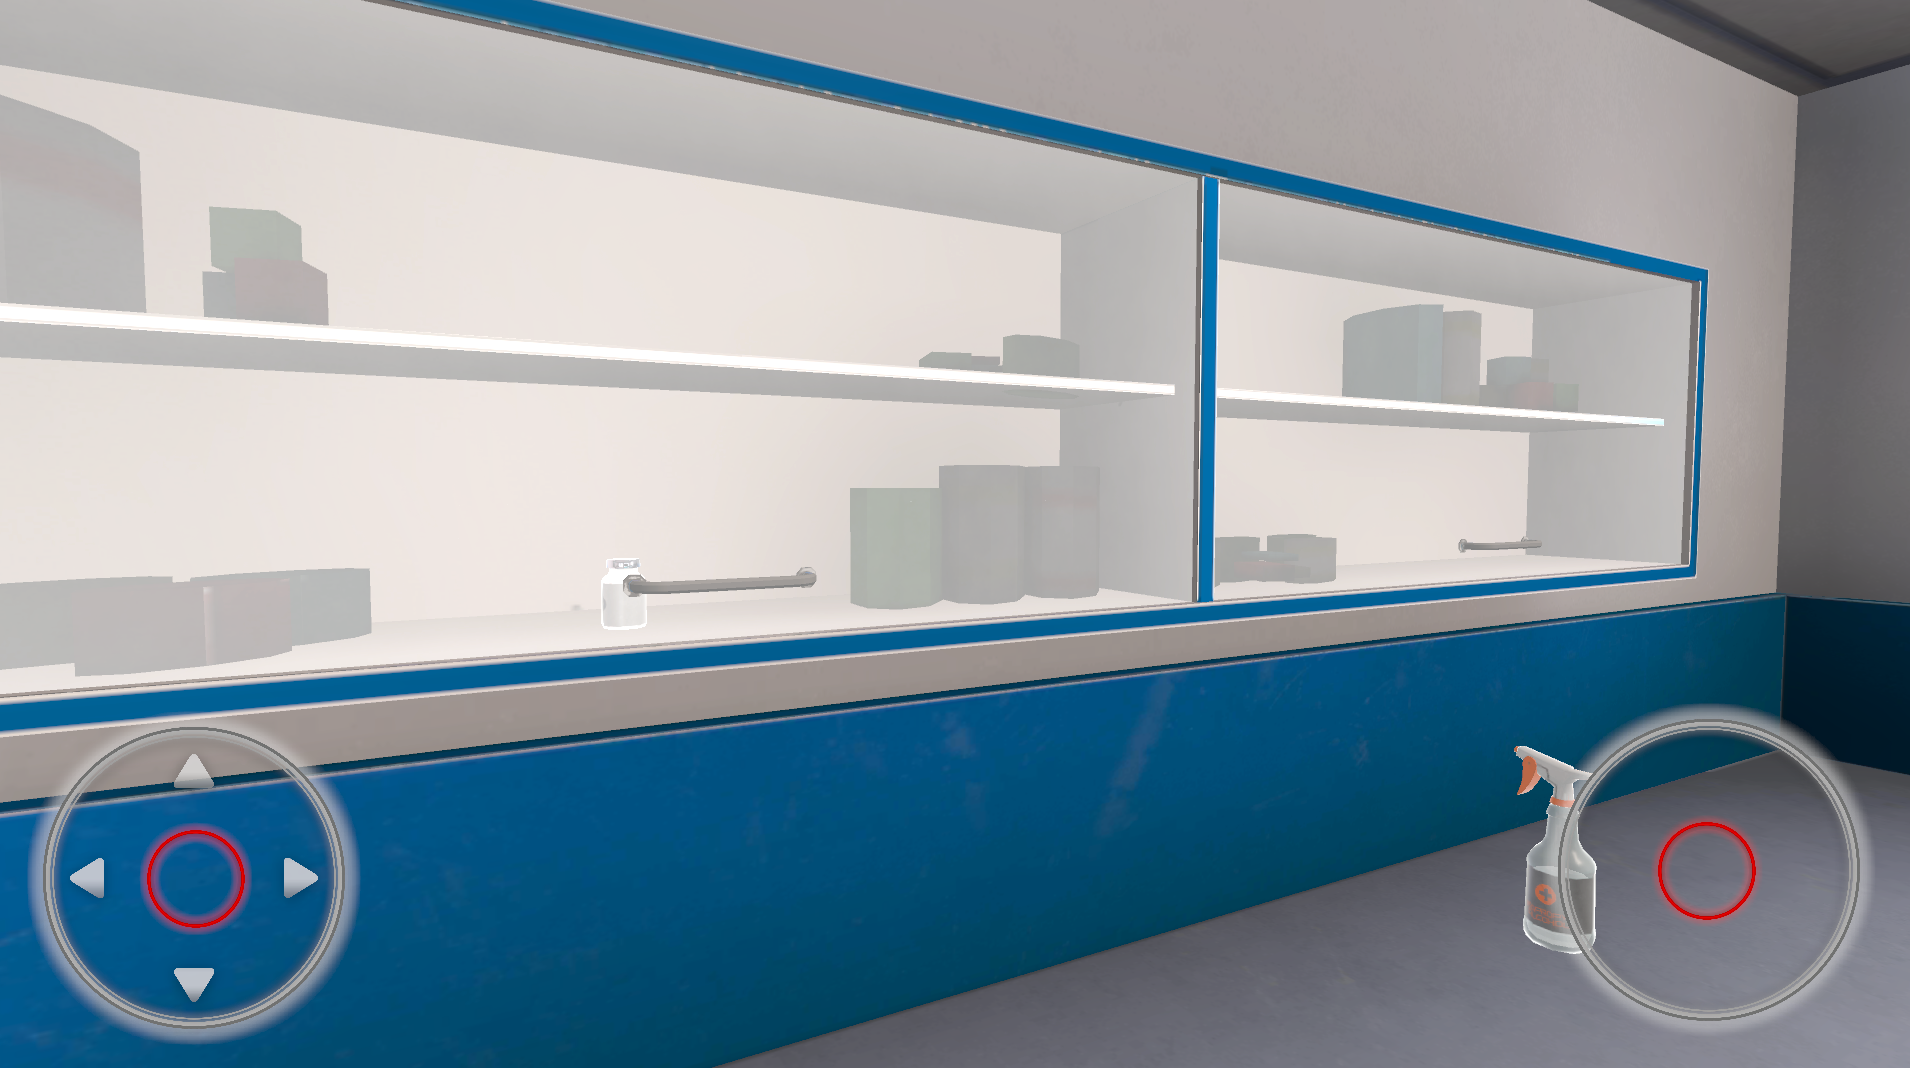
\includegraphics[width=0.5\textwidth, height=0.3\textheight]{Images/Tools and Medicine.png}
	\caption{Tools and Medicine}
	\label{fig:Tools and Medicine}
\end{figure}

\subsection{Tools Grabbing}
\text{Here are some actions performed before starting.}
\begin{figure}[h]
	\centering
	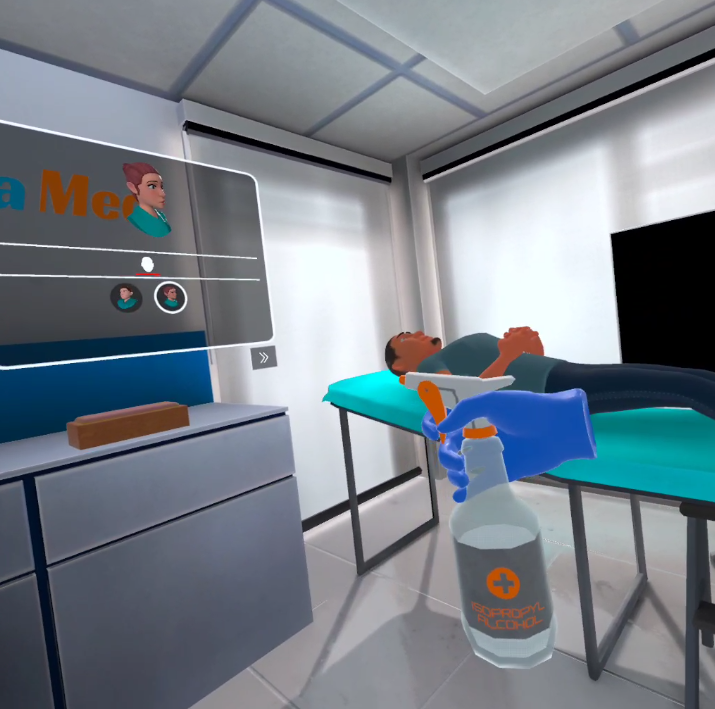
\includegraphics[width=0.5\textwidth, height=0.3\textheight]{Images/Grabbing Tool.png}
	\caption{Grabbing Tool}
	\label{fig:Grabbing-Tool}
\end{figure}

\subsubsection{Hands Washing}
\text{Here are some actions performed before starting.}
\begin{figure}[h]
	\centering
     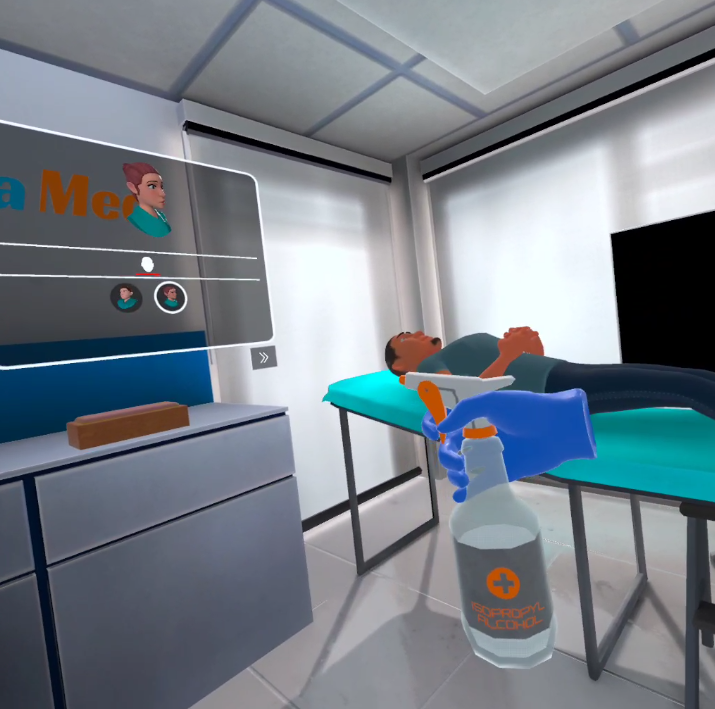
\includegraphics[width=0.5\textwidth, height=0.3\textheight]{Images/Washing hands.png}
	\caption{Hands Washing}
	\label{fig:Hands Washing}
\end{figure}

\subsubsection{Pour Alcohol}
\text{Here are some actions performed before starting.}
\begin{figure}[h]
	\centering
	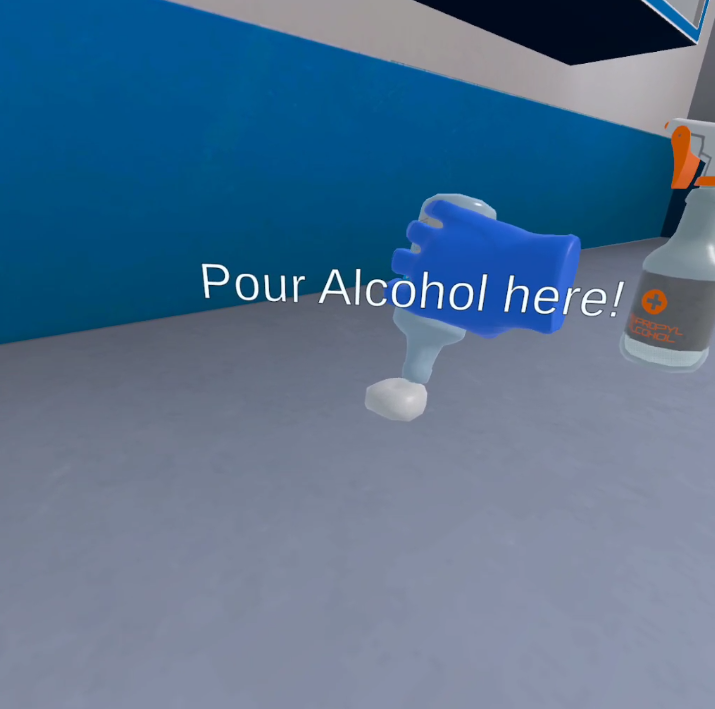
\includegraphics[width=0.5\textwidth, height=0.3\textheight]{Images/Pour Alcohol.png}
	\caption{Pour Alcohol}
	\label{fig:Pour-Alcohol}
\end{figure}

\subsubsection{Clean the injection site}
\text{Here are some actions performed before starting.}
\begin{figure}[h]
	\centering
	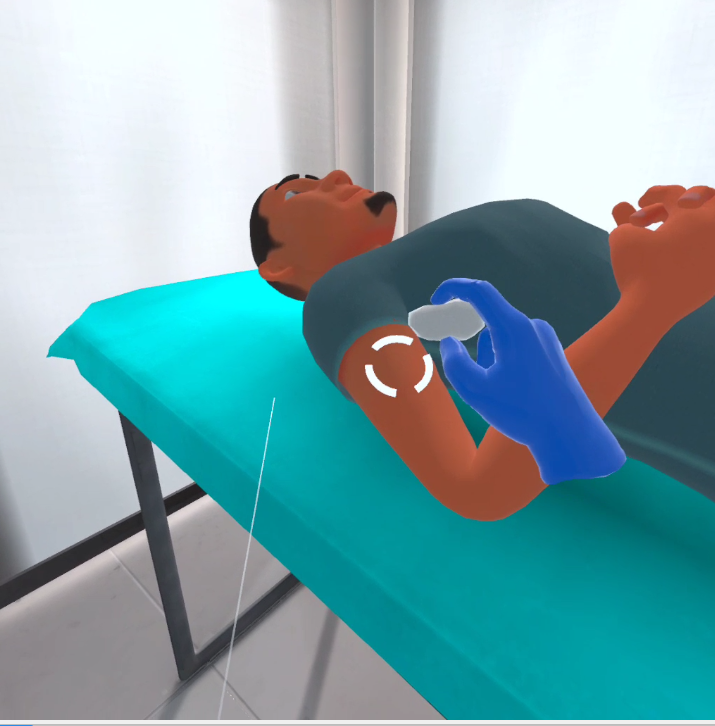
\includegraphics[width=0.5\textwidth, height=0.3\textheight]{Images/Clean the injection site.png}
	\caption{Clean the injection site}
	\label{fig:Clean the injection site}
\end{figure}

\subsubsection{Dispose the Cotton}
\text{Here are some actions performed before starting.}
\begin{figure}[h]
	\centering
	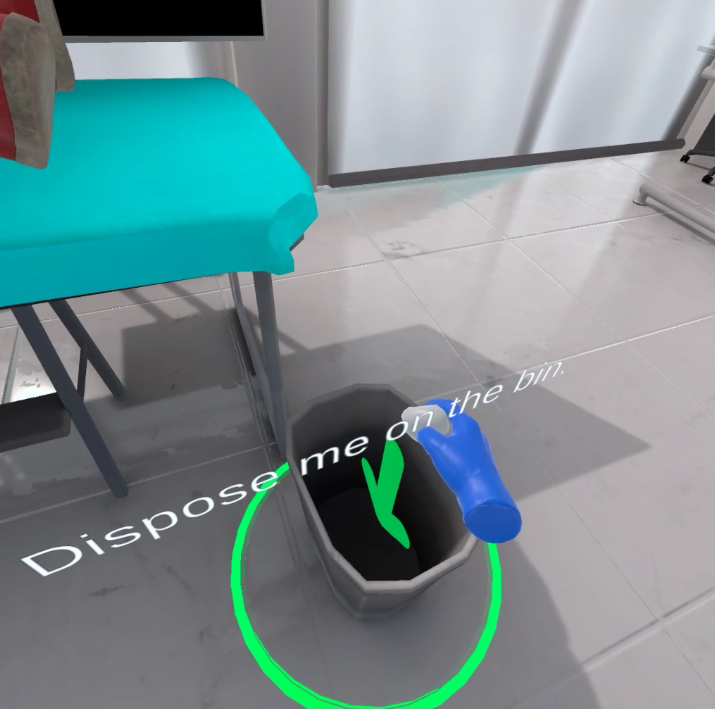
\includegraphics[width=0.5\textwidth, height=0.3\textheight]{Images/Dispose the Cotton.png}
	\caption{Dispose the Cotton}
	\label{fig:Dispose the Cotton}
\end{figure}

\subsubsection{Picking the injection}
\text{Here are some actions performed before starting.}
\begin{figure}[h]
	\centering
	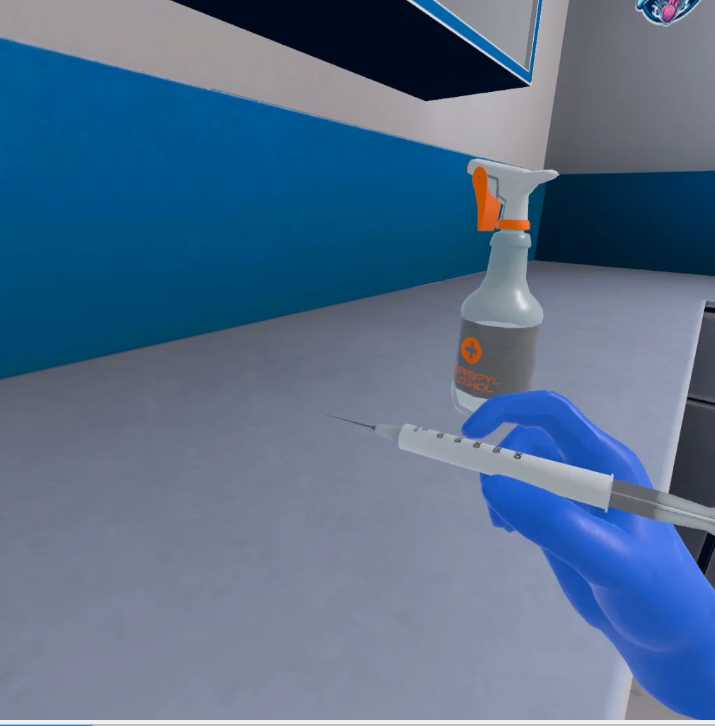
\includegraphics[width=0.5\textwidth, height=0.3\textheight]{Images/Picking the injection.png}
	\caption{Picking the injection}
	\label{fig:Picking the injection}
\end{figure}

\subsubsection{Inject the medication}
\text{Here are some actions performed before starting.}
\begin{figure}[h]
	\centering
	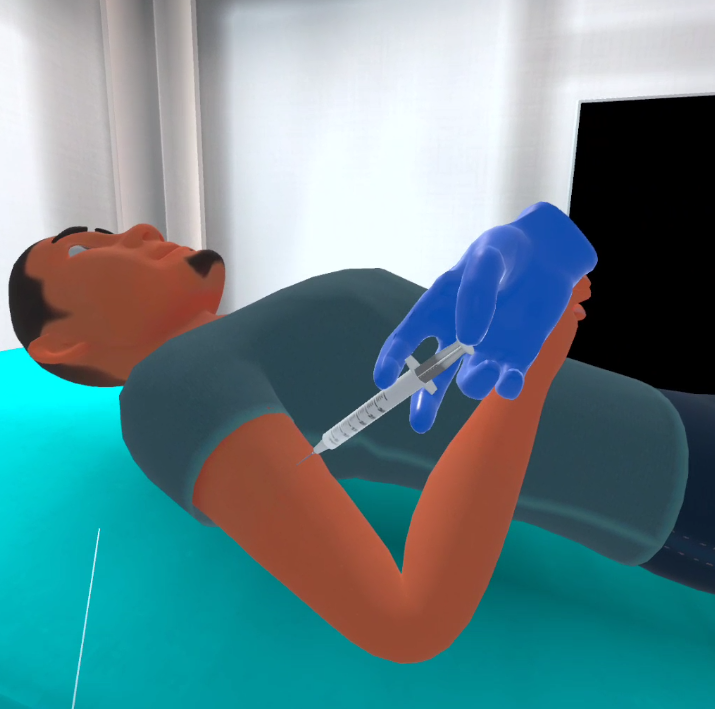
\includegraphics[width=0.5\textwidth, height=0.3\textheight]{Images/Inject the medication.png}
	\caption{Inject the medication}
	\label{fig:Inject the medication}
\end{figure}

\subsubsection{Applying Cut on Body}
\text{Here are some actions performed before starting.}
\begin{figure}[h]
	\centering
	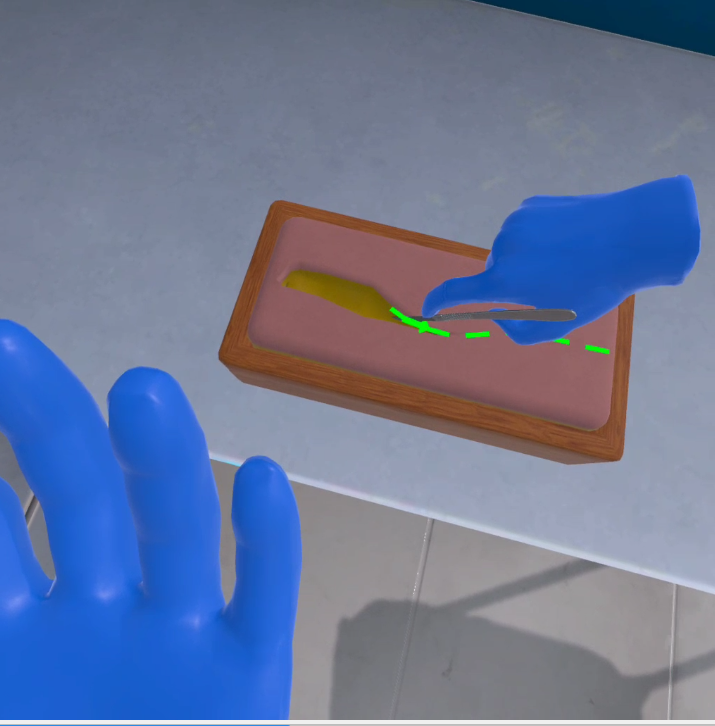
\includegraphics[width=0.5\textwidth, height=0.3\textheight]{Images/Applying Cut on Body.png}
	\caption{Applying Cut on Body}
	\label{fig:Applying Cut on Body}
\end{figure}
\newpage
\subsubsection{Objects Movement}
\text{Here are some actions performed before starting.}
\begin{figure}[h]
	\centering
	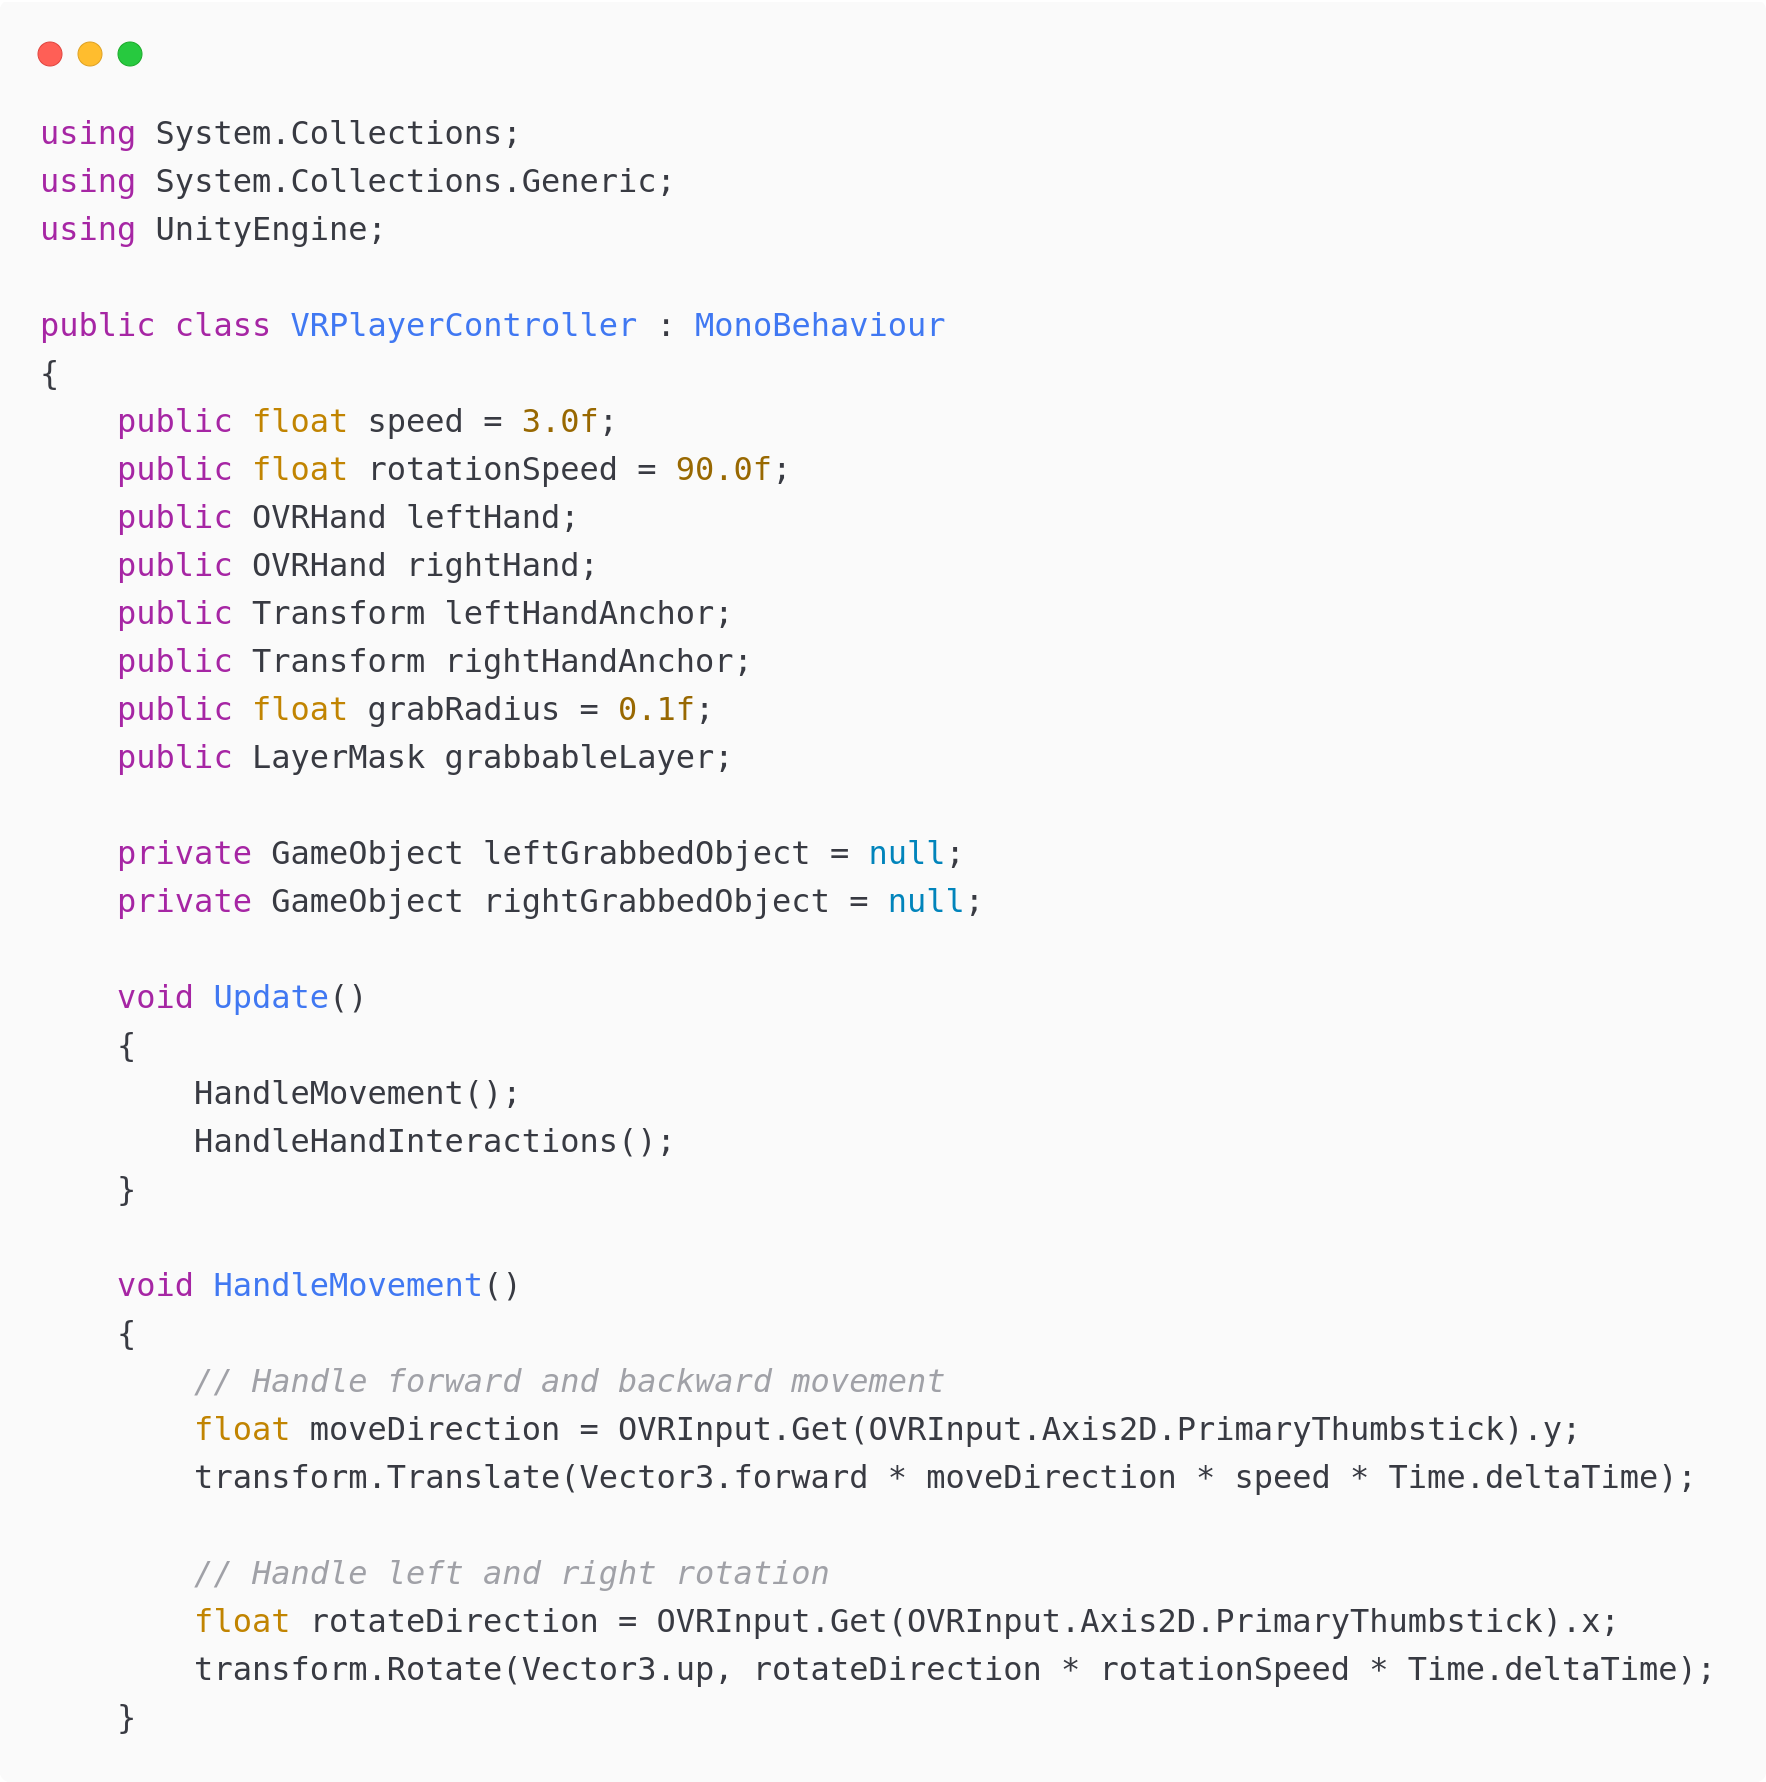
\includegraphics[width=1\textwidth, height=0.7\textheight]{Images/playerp1.png}
	\caption{user part 1}
	\label{fig:Grabbing-Tool}
\end{figure}
\newpage
\begin{figure}[h] 
	\centering
	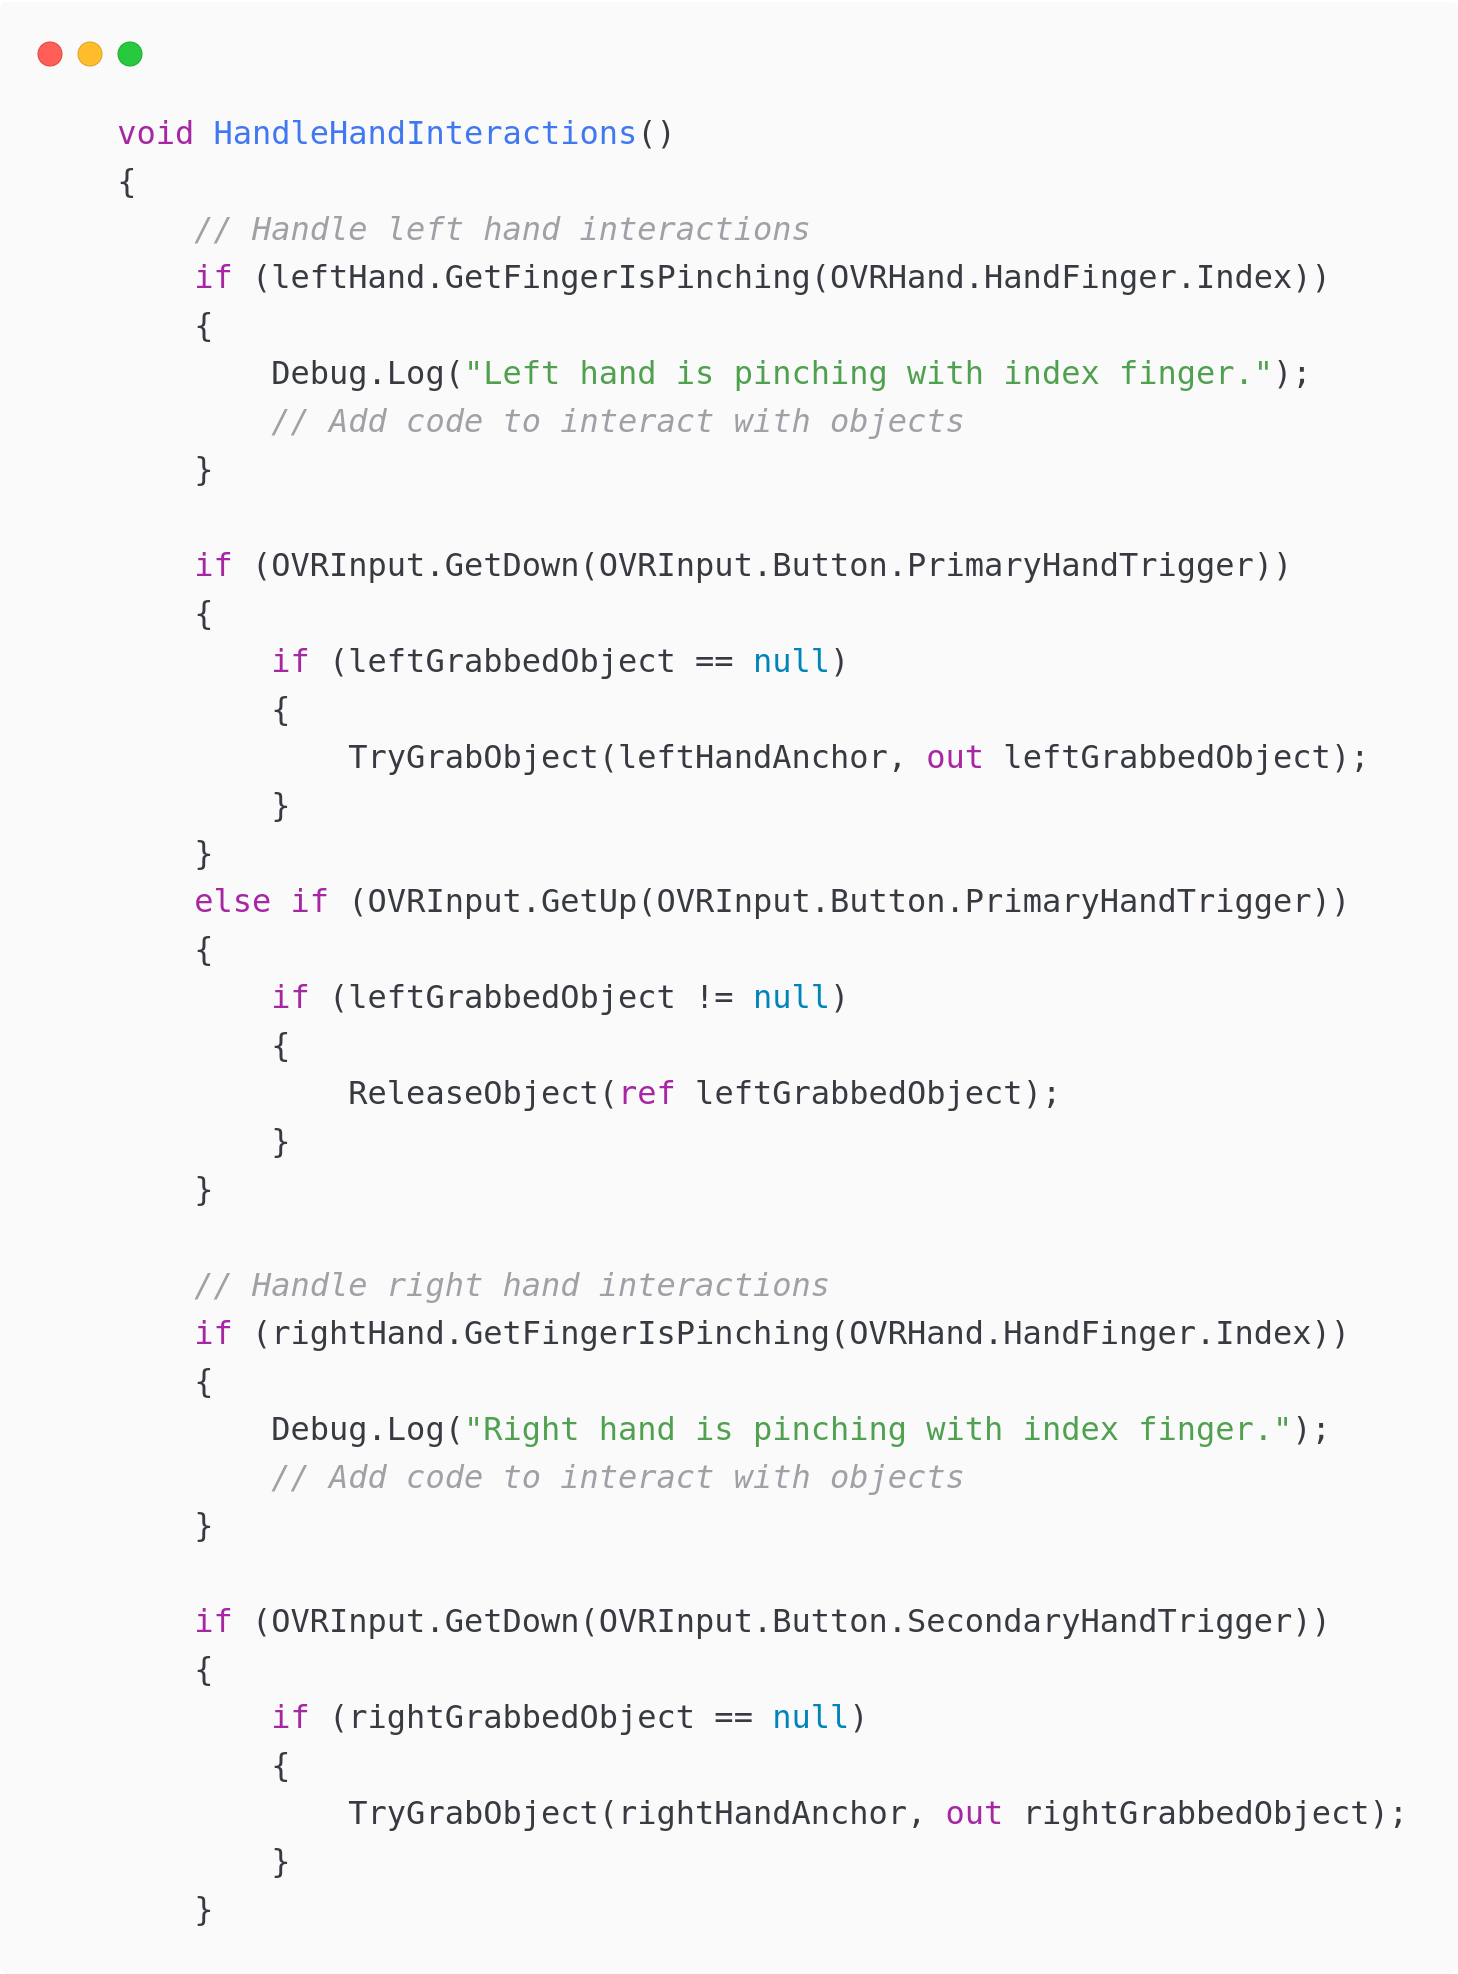
\includegraphics[width=1\textwidth, height=0.7\textheight]{Images/playerp2.png}
	\caption{user part 2}
	\label{fig:Hands Washing}
\end{figure}

\newpage
\begin{figure}[h] 
	\centering
	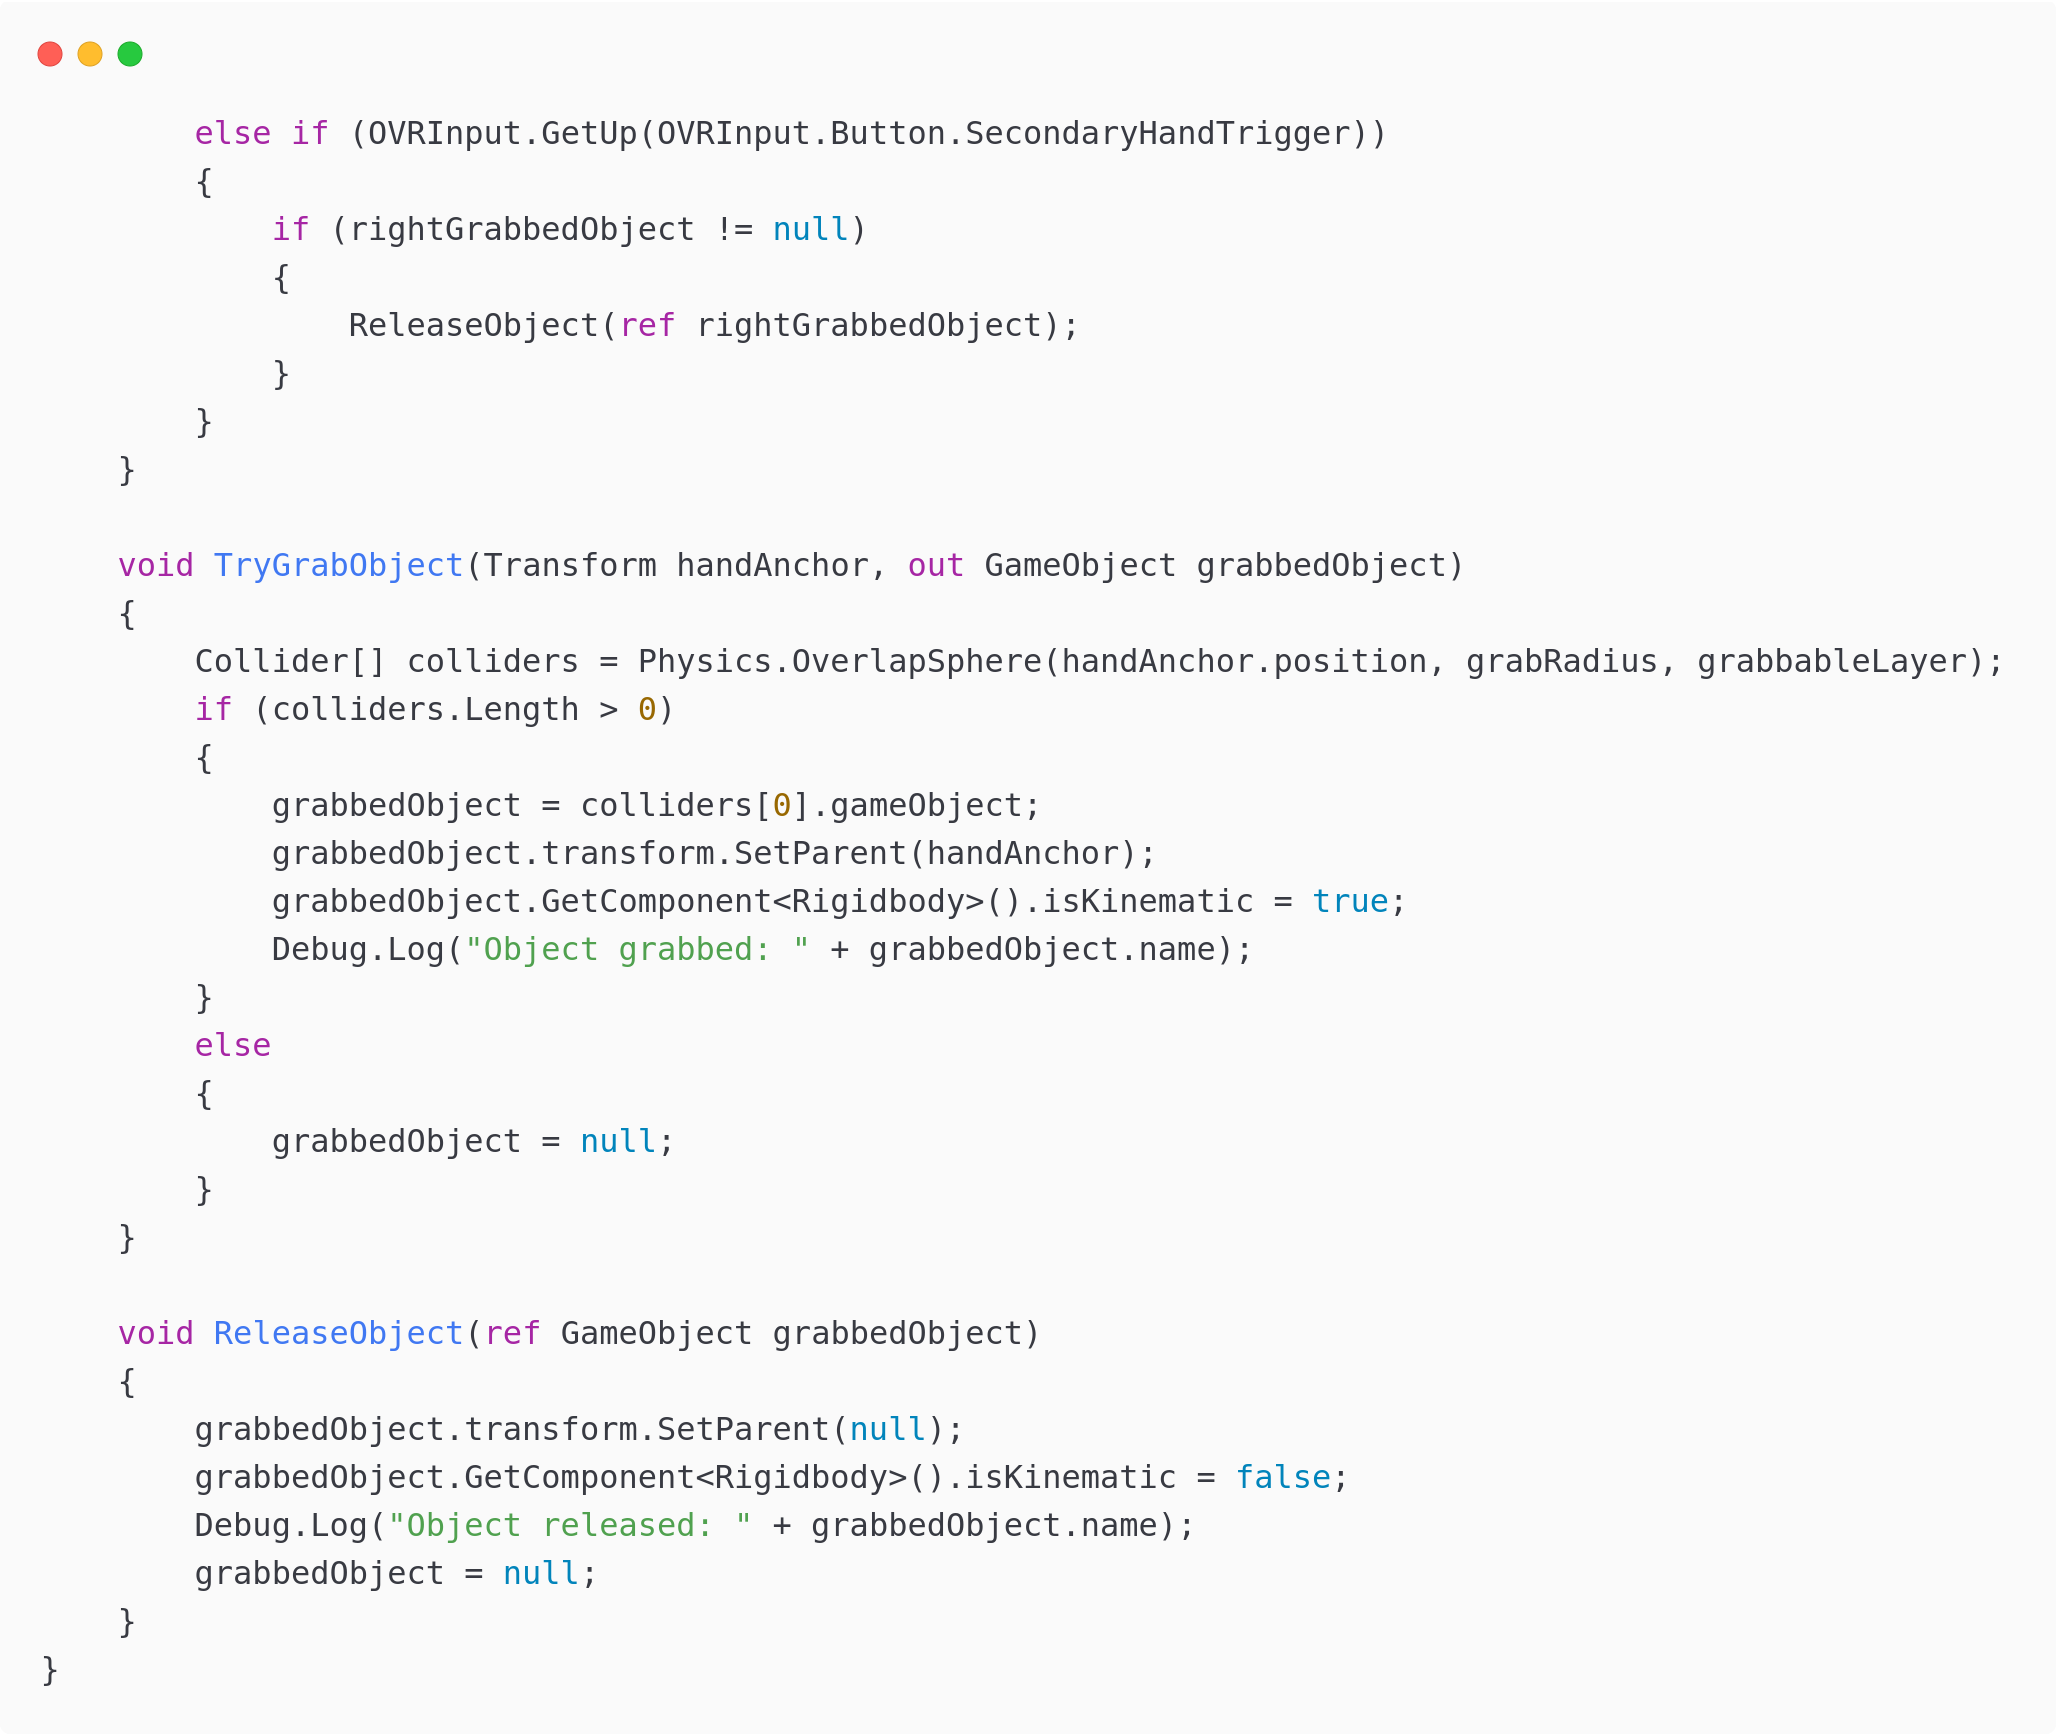
\includegraphics[width=1\textwidth, height=0.7\textheight]{Images/playerp3.png}
	\caption{user part 3}
	\label{fig:Hands Washing}
\end{figure}
\newpage
\begin{figure}[h]
	\centering
	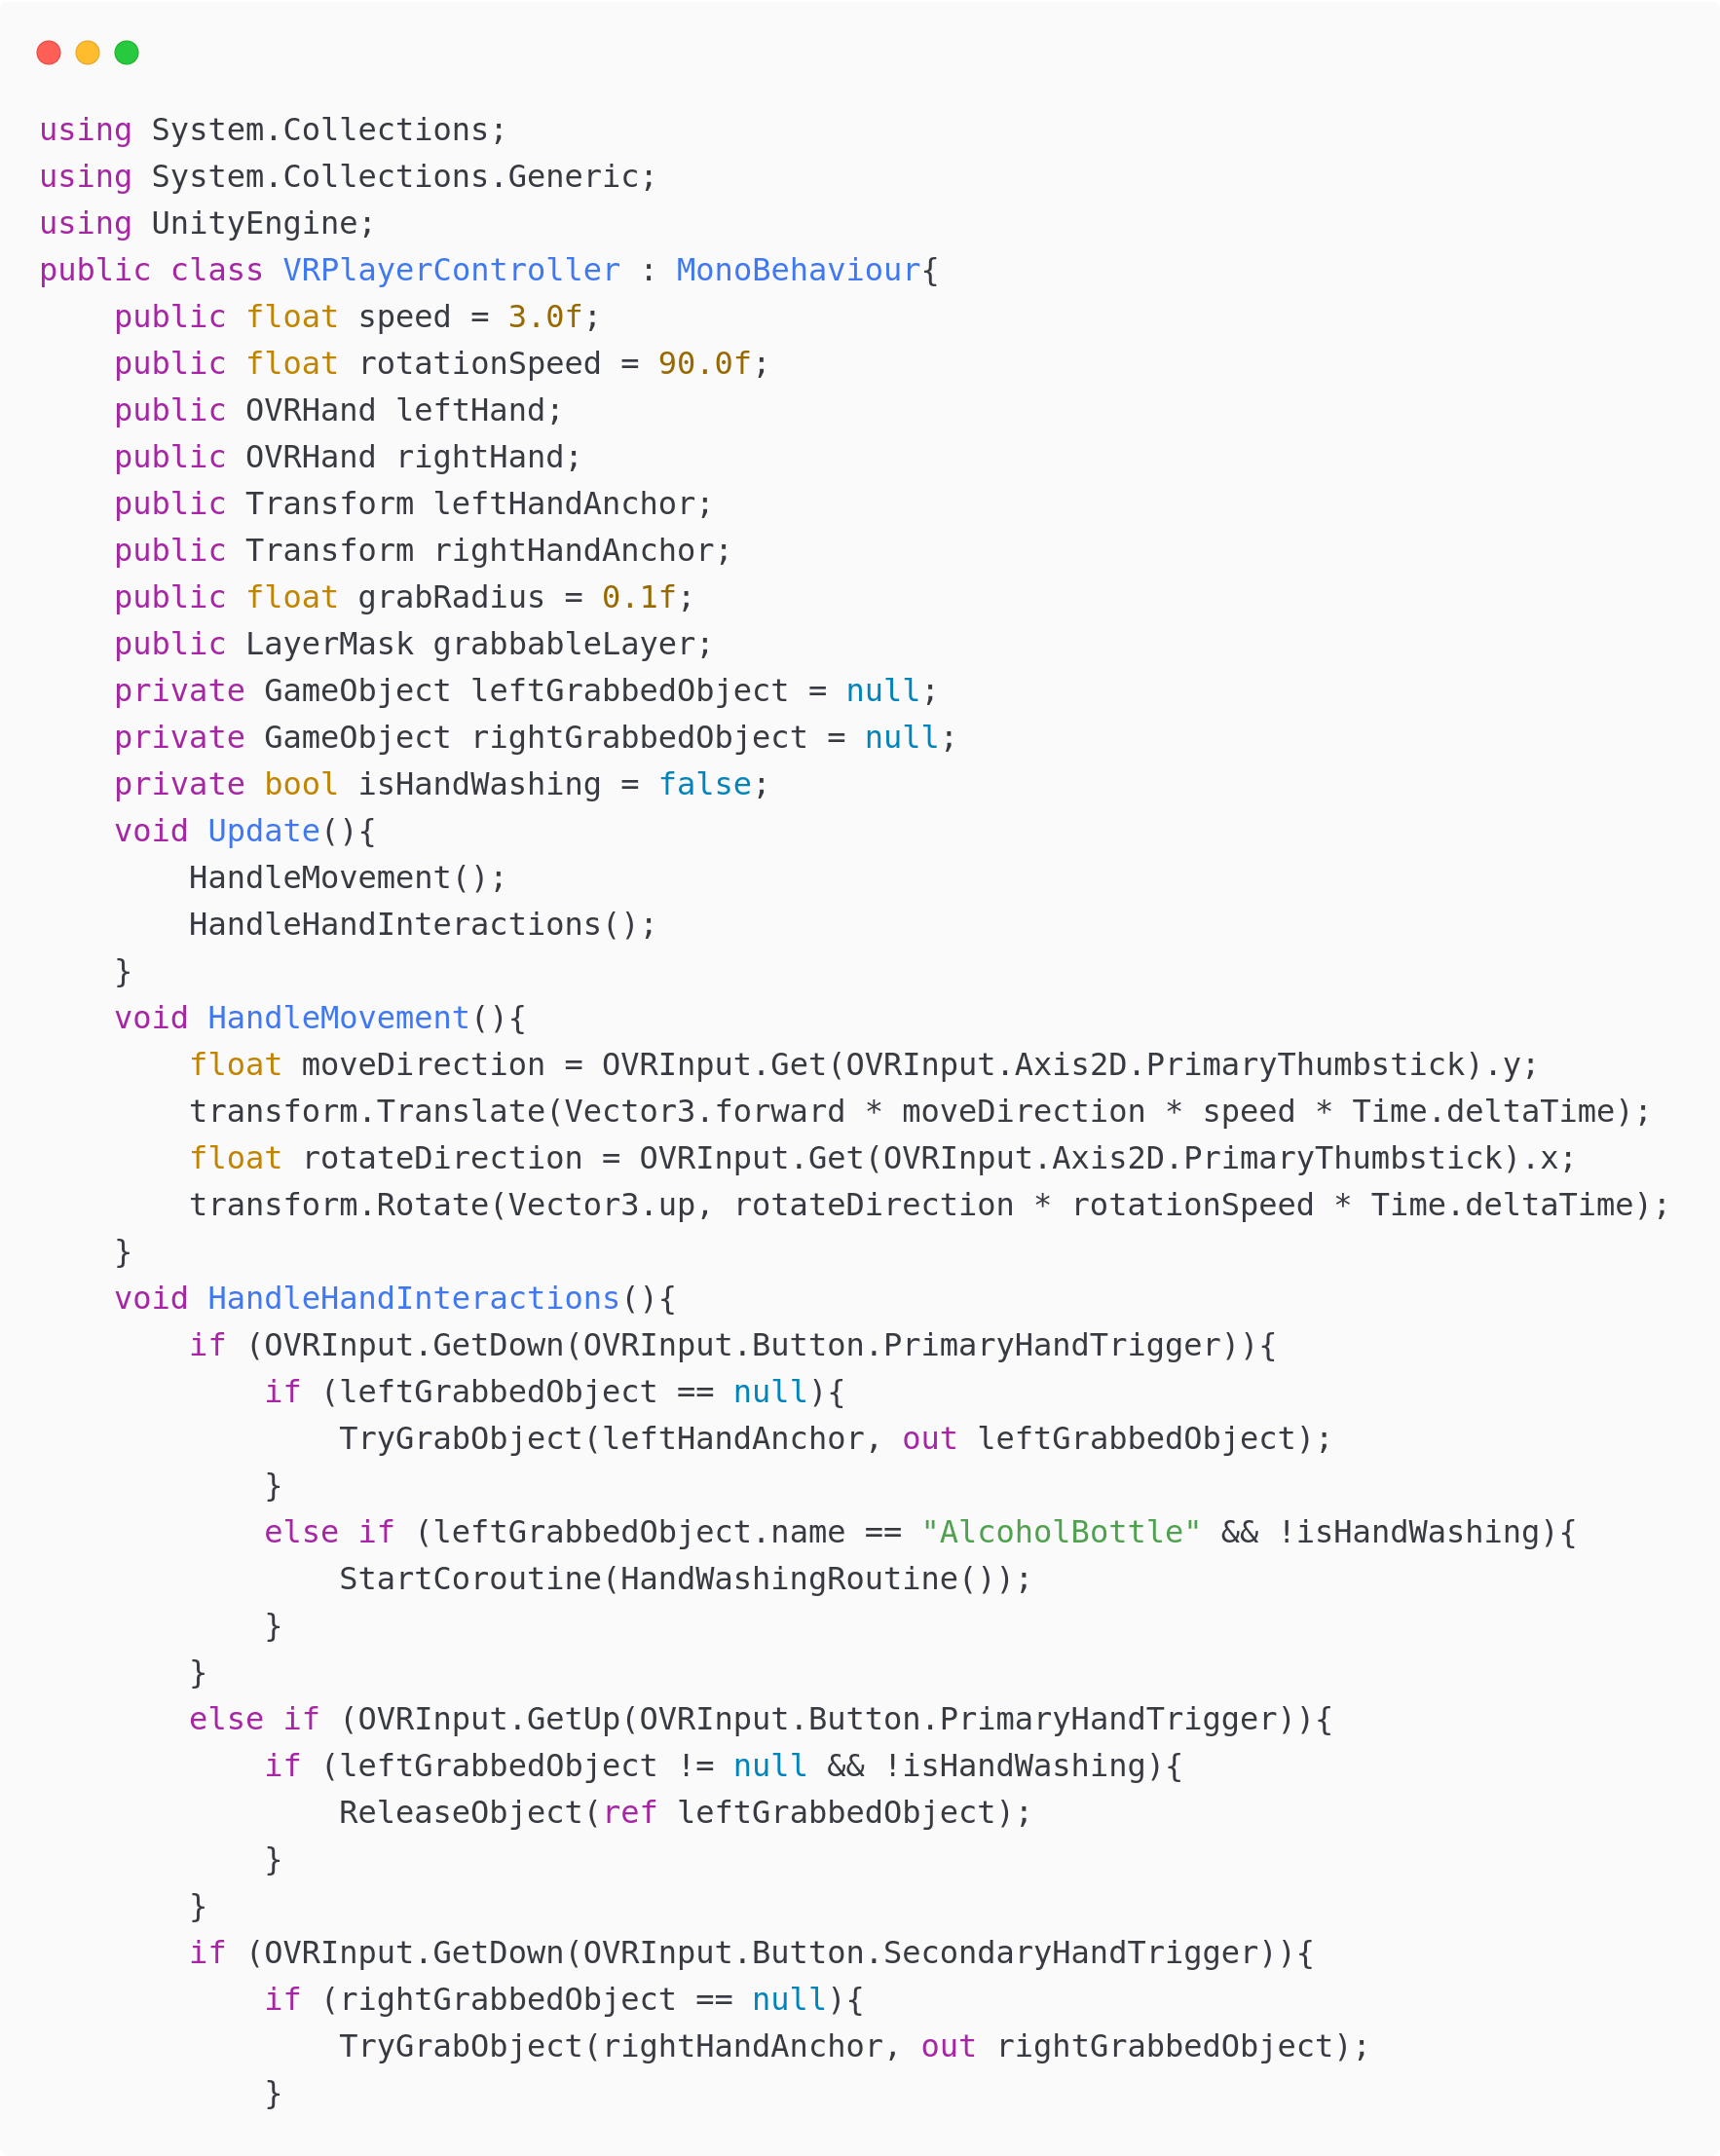
\includegraphics[width=1\textwidth, height=0.7\textheight]{Images/pore alcohol1.png}
	\caption{Pore Alcohol for Hands Washing Part 1}
	\label{fig:Grabbing-Tool}
\end{figure}
\newpage
\begin{figure}[h] 
	\centering
	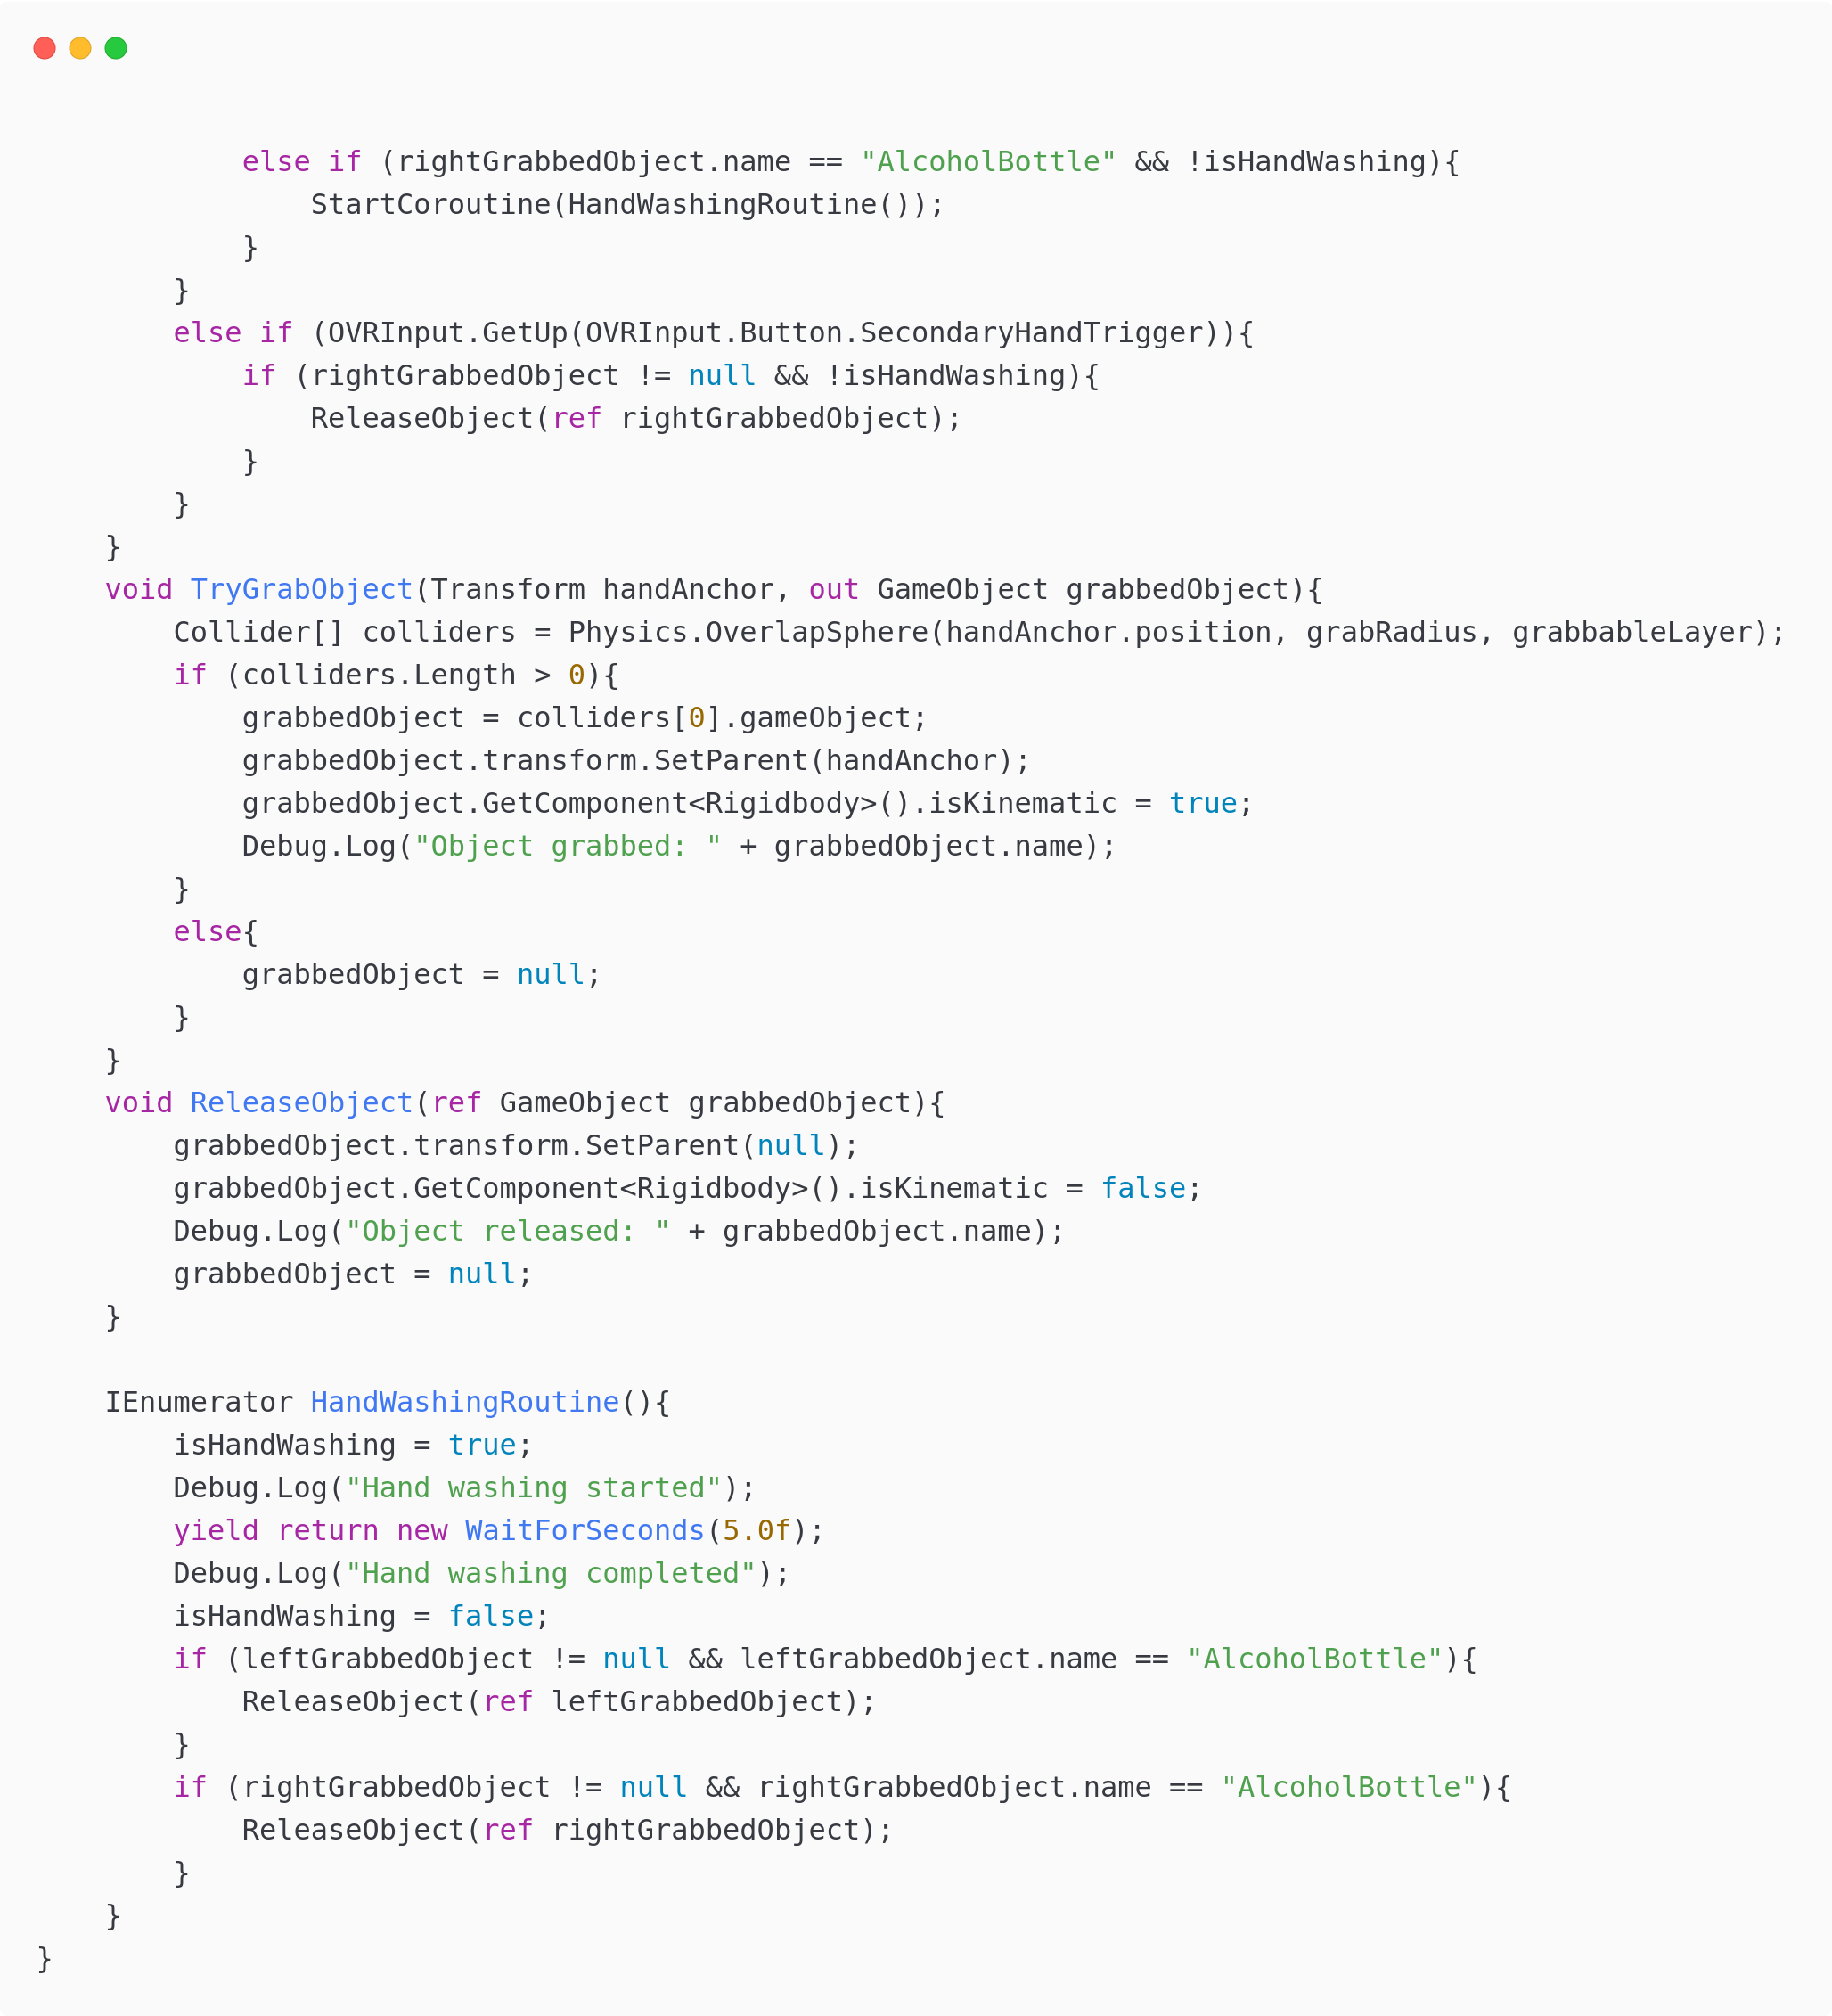
\includegraphics[width=1\textwidth, height=0.7\textheight]{Images/pore alcohol2.png}
	\caption{Pore Alcohol for Hands Washing Part 2}
	\label{fig:Hands Washing}
\end{figure}

\newpage
\begin{figure}[h] 
	\centering
	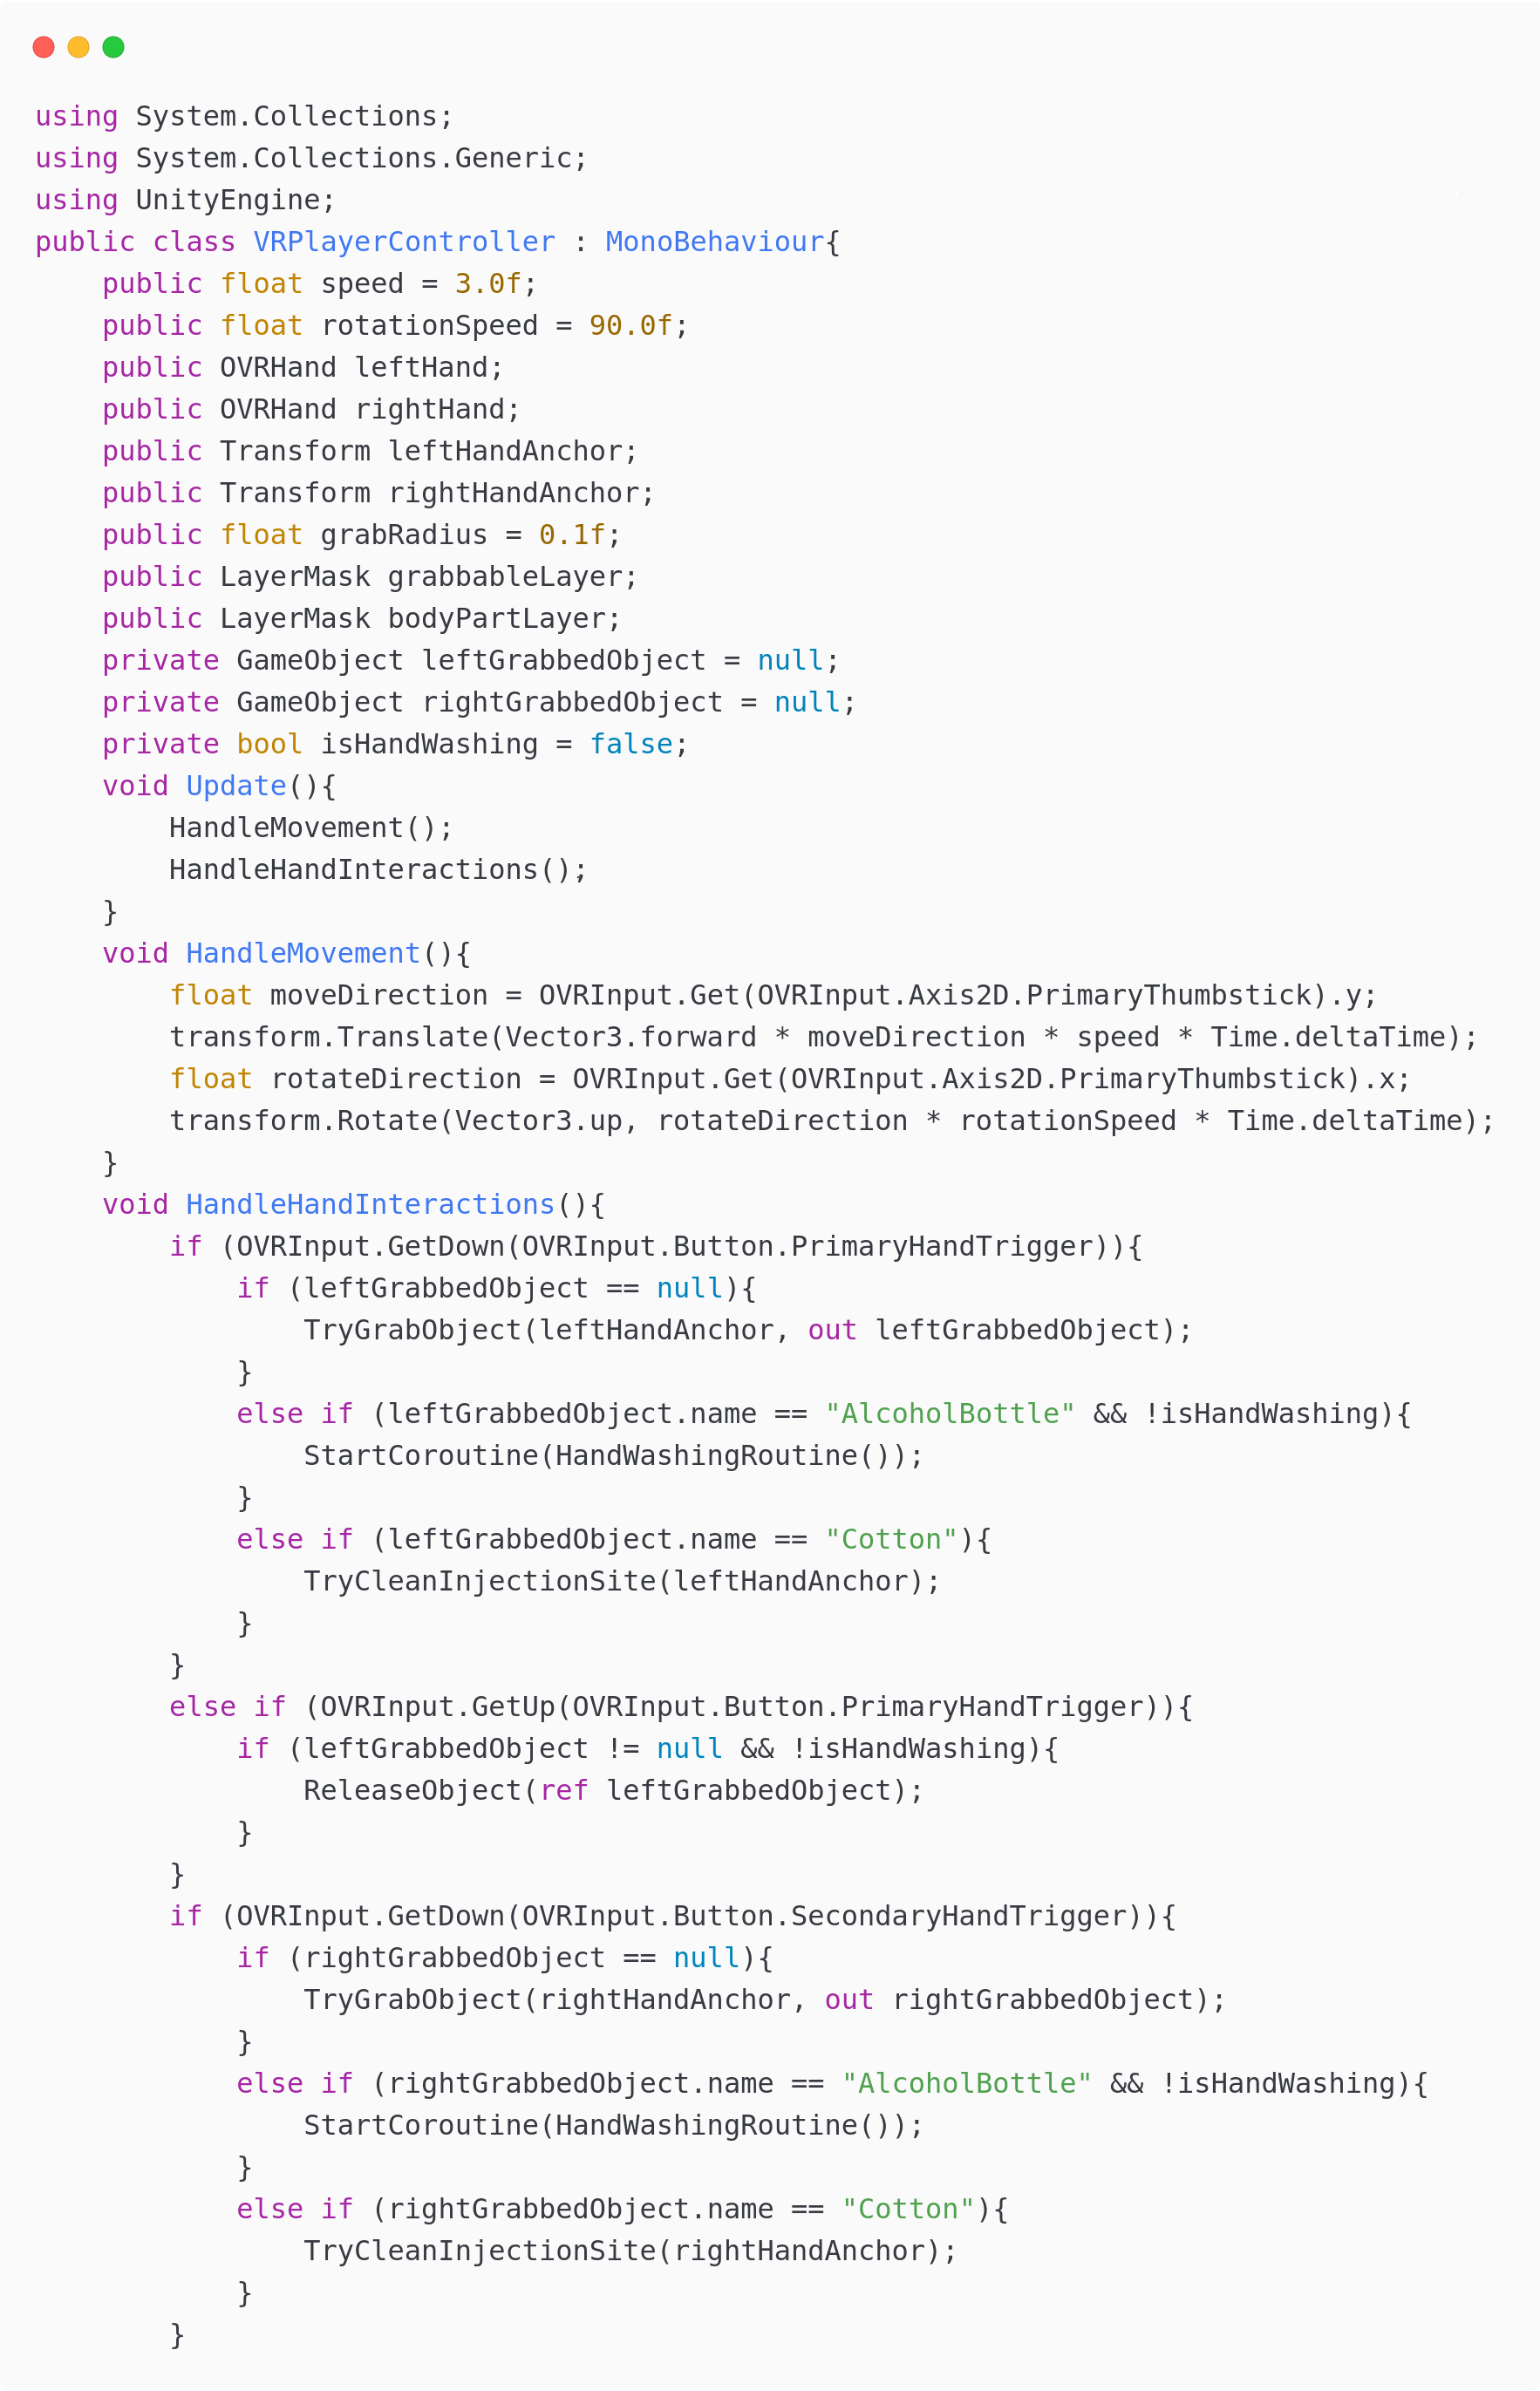
\includegraphics[width=1\textwidth, height=0.7\textheight]{Images/cleaning1.png}
	\caption{Cleaning Injection Site Part 1}
	\label{fig:Hands Washing}
\end{figure}
\newpage
\begin{figure}[h] 
	\centering
	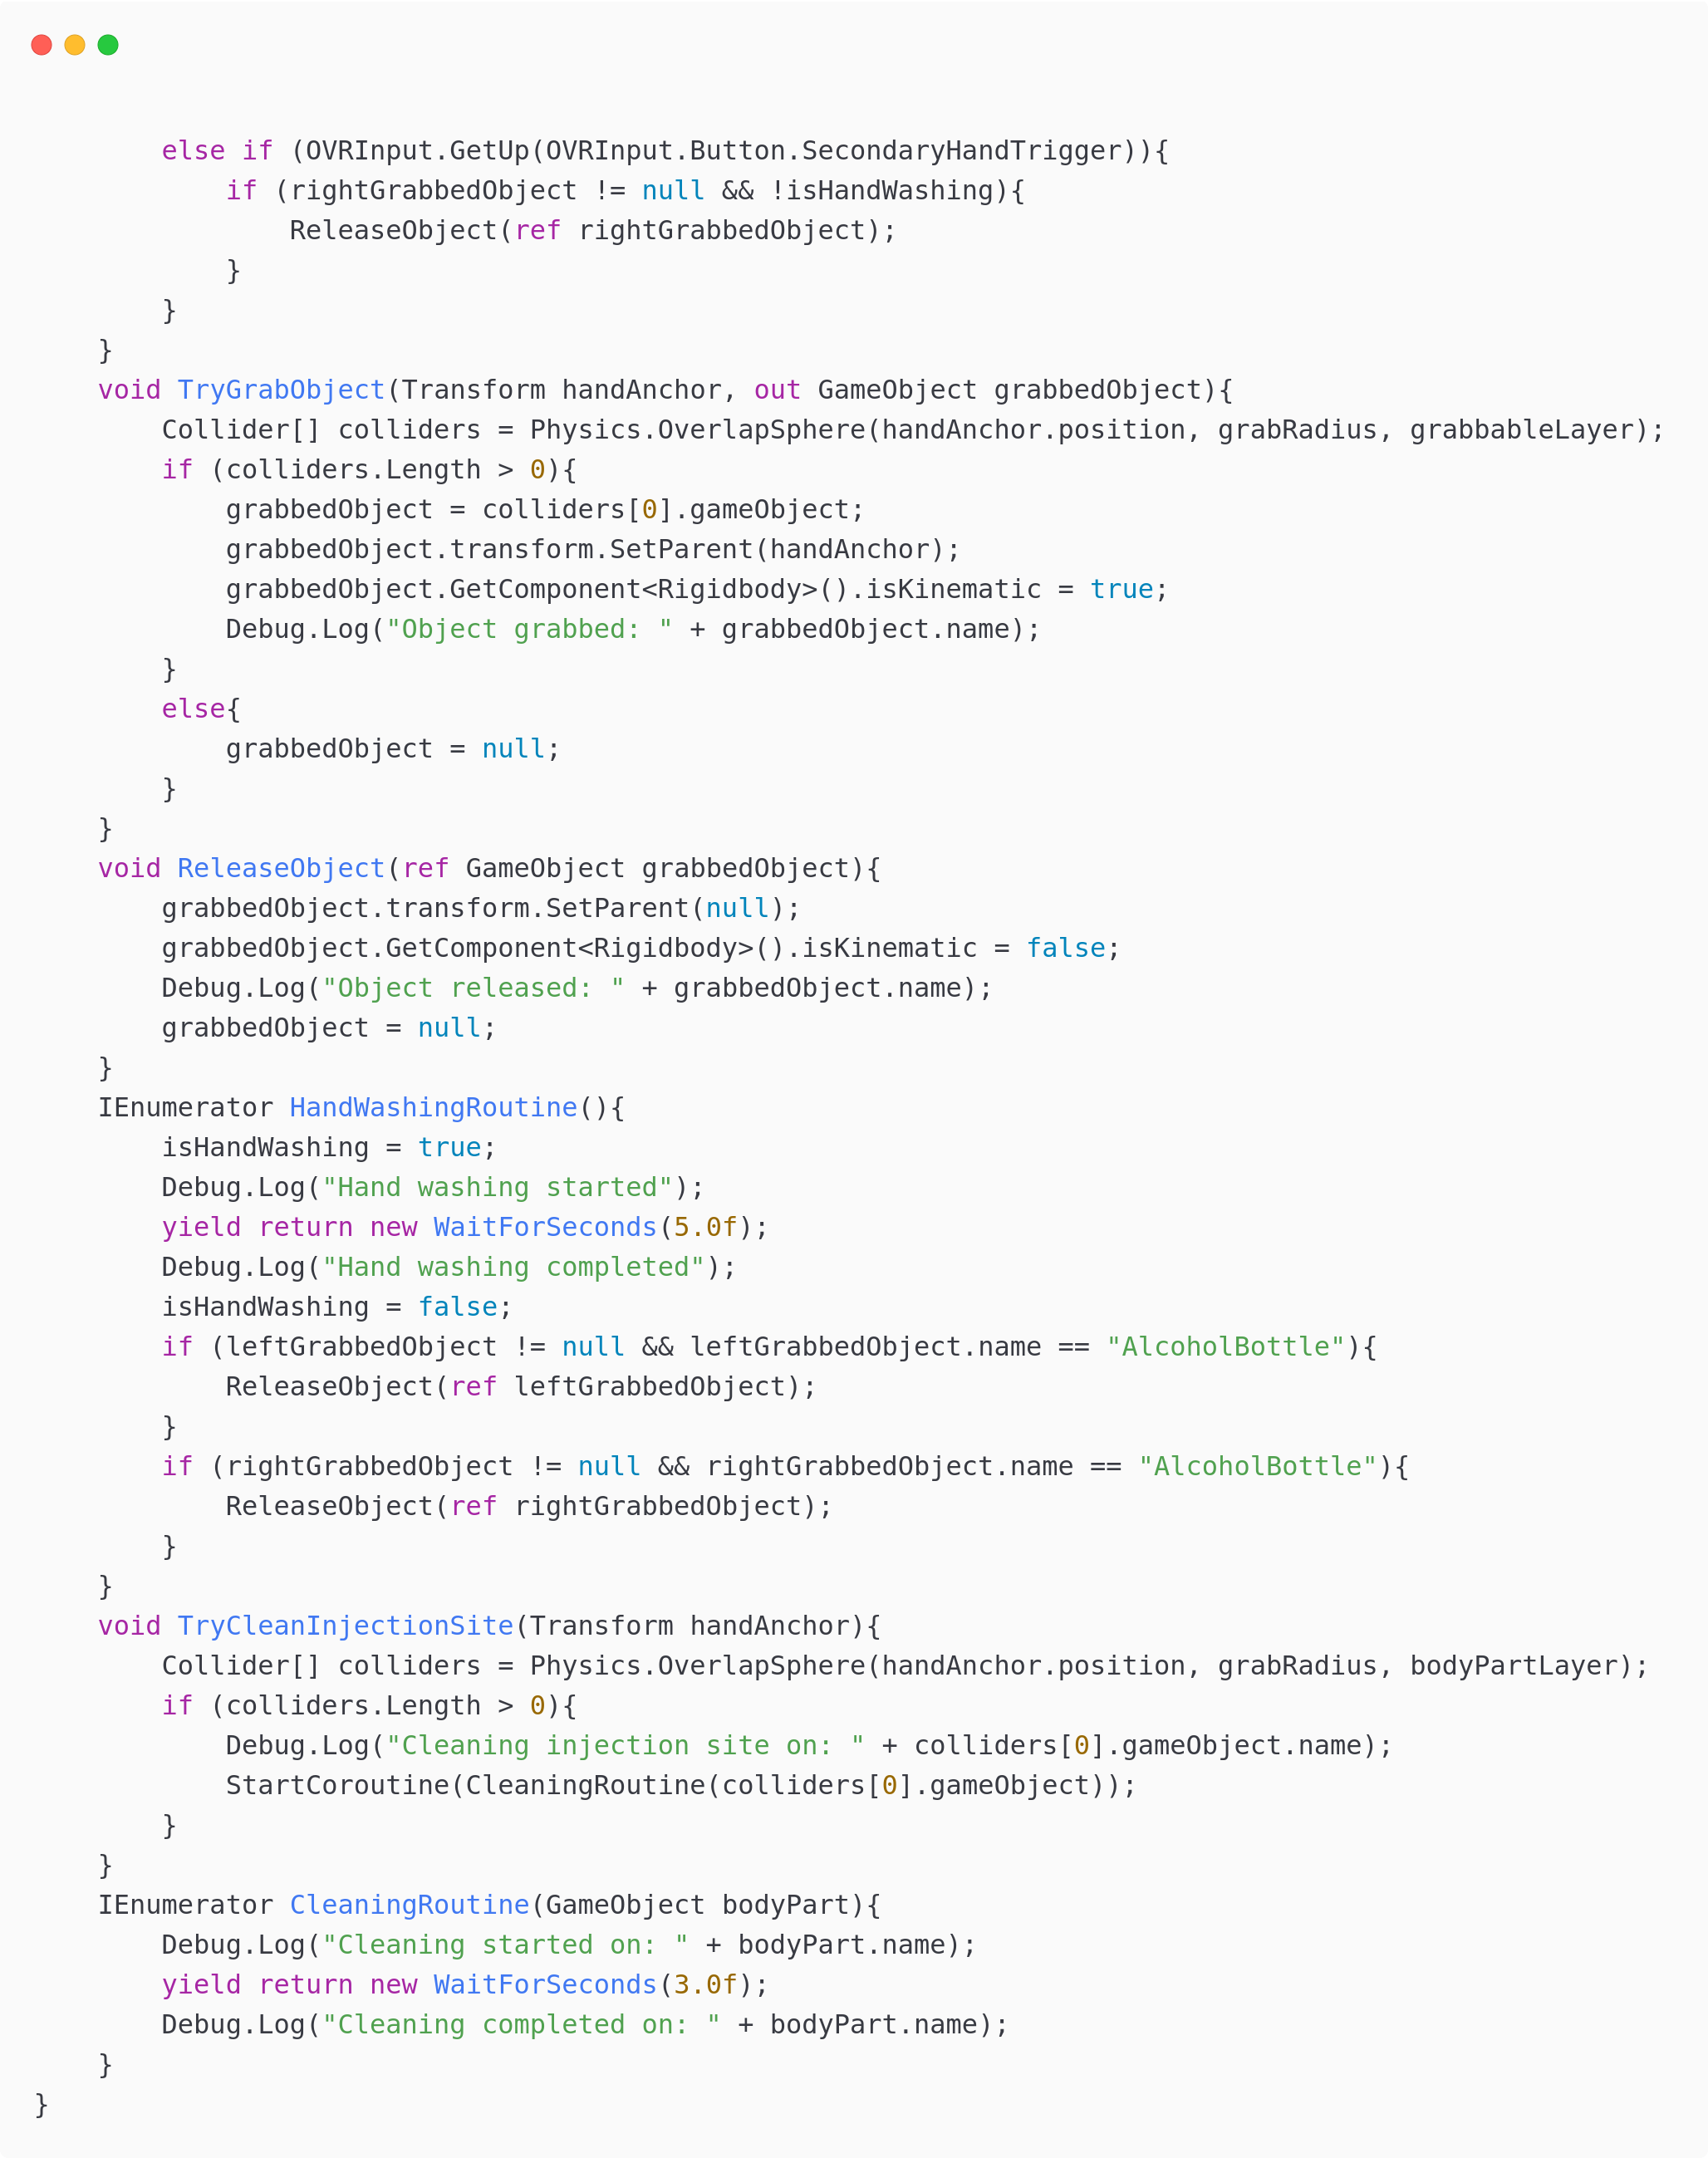
\includegraphics[width=1\textwidth, height=0.7\textheight]{Images/cleaning2.png}
	\caption{Cleaning Injection Site Part 2}
	\label{fig:Hands Washing}
\end{figure}

\newpage
\begin{figure}[h] 
	\centering
	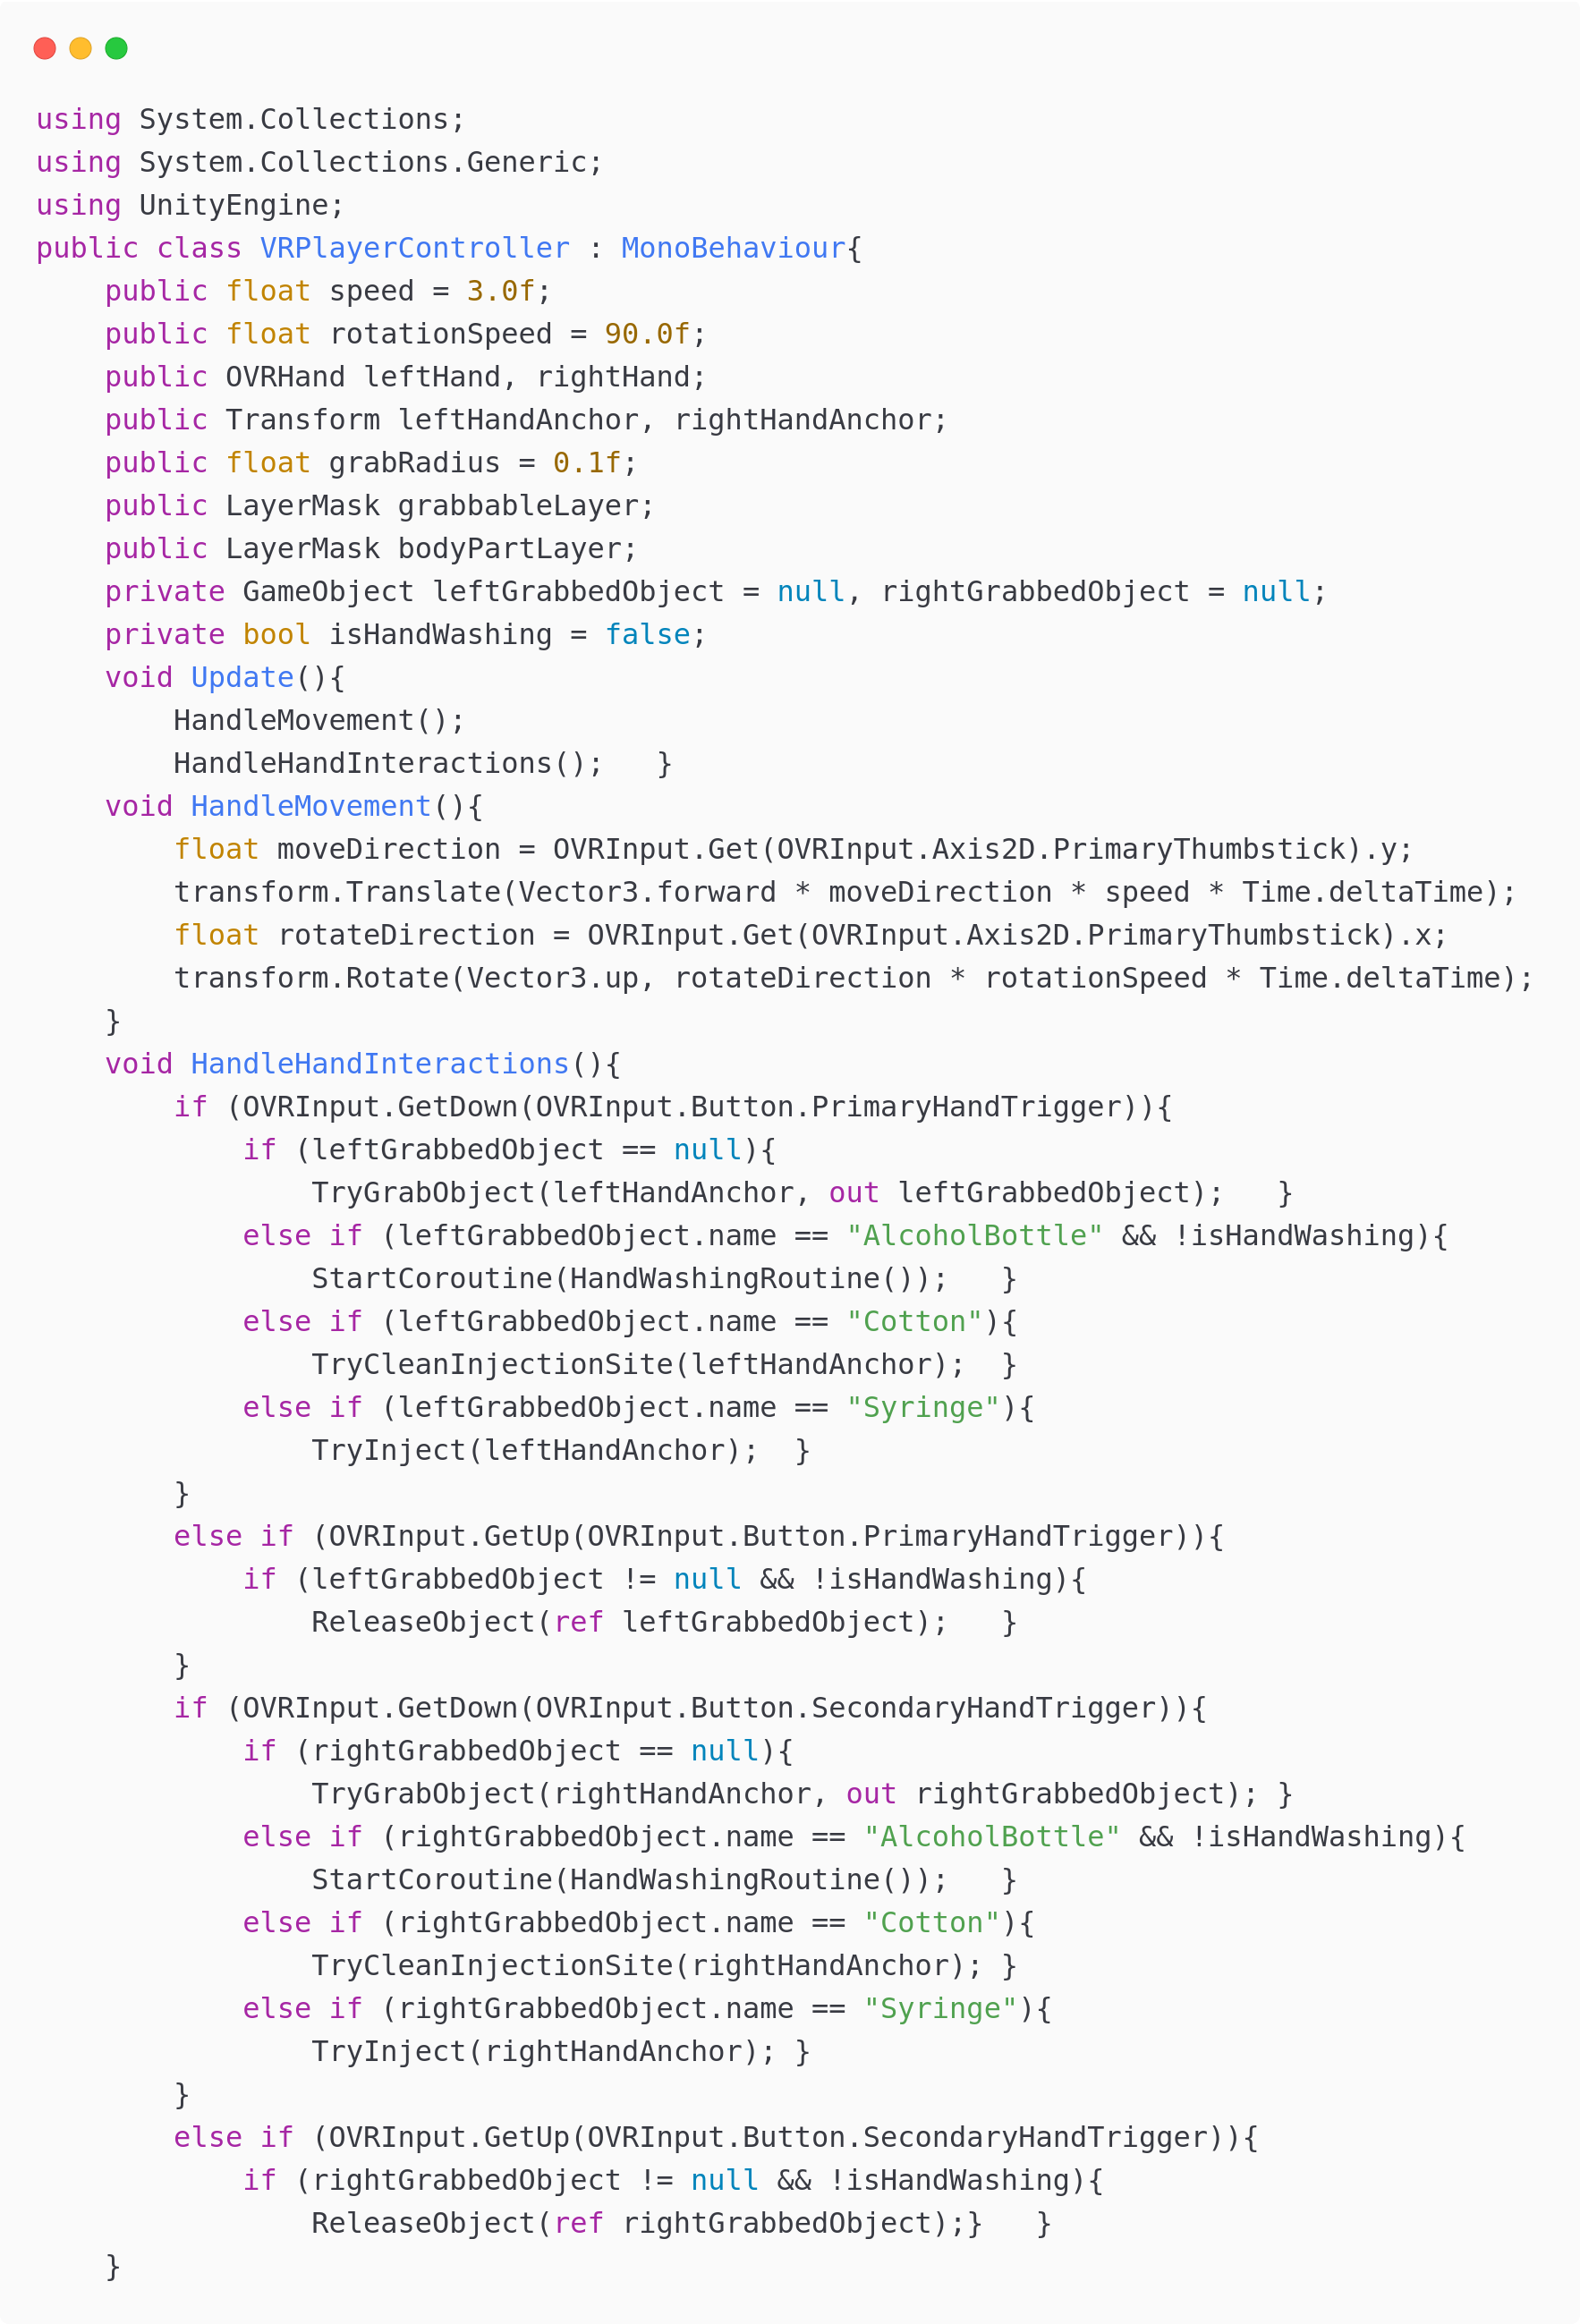
\includegraphics[width=1\textwidth, height=0.7\textheight]{Images/inject1.png}
	\caption{inject2}
	\label{fig:Hands Washing}
\end{figure}
\newpage
\begin{figure}[h] 
	\centering
	\includegraphics[width=1\textwidth, height=0.7\textheight]{Images/inject2.png}
	\caption{inject2}
	\label{fig:Hands Washing}
\end{figure}

\section{SVN or GitHub}
We have uploaded on GitHub. Here is the GitHub link: \\
\href{https://github.com/Daudsarfraz/MetaMed}{https://github.com/Daudsarfraz/MetaMed}